\documentclass{article}
\usepackage[english]{babel}
\usepackage[margin=1in]{geometry}
\usepackage{array}
\newcolumntype{L}{>{\raggedright\arraybackslash}X}
\usepackage{tocloft}
\usepackage{hyperref}
\usepackage{bookmark}
\usepackage{makeidx}
\usepackage{amsmath}
\usepackage{graphicx}
\usepackage{listings}
\usepackage{xcolor}
\usepackage{float}

\usepackage{booktabs}% http://ctan.org/pkg/booktabs
\newcommand{\tabitem}{~~\llap{\textbullet}~~}

\definecolor{codegreen}{rgb}{0,0.6,0}
\definecolor{codegray}{rgb}{0.5,0.5,0.5}
\definecolor{codepurple}{rgb}{0.58,0,0.82}
\definecolor{backcolour}{rgb}{0.95,0.95,0.92}

\lstdefinestyle{mystyle}{
	backgroundcolor=\color{backcolour},   
	commentstyle=\color{codegreen},
	keywordstyle=\color{magenta},
	numberstyle=\tiny\color{codegray},
	stringstyle=\color{codepurple},
	basicstyle=\ttfamily\footnotesize,
	breakatwhitespace=false,         
	breaklines=true,                 
	captionpos=b,                    
	keepspaces=true,                 
	numbers=left,                    
	numbersep=5pt,                  
	showspaces=false,                
	showstringspaces=false,
	showtabs=false,                  
	tabsize=2
}
\lstset{style=mystyle}


\title{University of Calabria, DIMES\\High Level Synthesis of Digital Systems\\2023-2024\\Prof.ssa PERRI\\Prof. FRUSTACI\\Sparse Matrix Vector Multiplication Analysis}
\author{Giorgio Ubbriaco \\ 247284 \\ bbrgrg00h11d086x@studenti.unical.it}
\date{June 2024}

\begin{document}
	\maketitle
	\renewcommand{\contentsname}{Index}
	\tableofcontents
	\newpage
	
	\lstlistoflistings
	\listoffigures
	\listoftables
	\newpage
	
	\section{Introduction}
	\subsection{Sparse Matrix}
Nell'analisi numerica, una \textbf{matrice sparsa} è una matrice in cui la maggior parte degli elementi presenta un valore nullo. Non esiste una definizione rigorosa della proporzione di elementi a valore nullo affinché una matrice possa essere considerata sparsa. Al contrario, se la maggior parte degli elementi è non nulla, allora la matrice è considerata densa.
\\
Una matrice è tipicamente memorizzata come un array bidimensionale. Ogni voce della matrice rappresenta un elemento $a_{i,j}$ e vi si accede tramite l'indice di riga i e l'indice di colonna j. Per una matrice m × n, la quantità di memoria necessaria per memorizzare la matrice in questo formato è proporzionale a m × n (senza considerare che è necessario memorizzare anche le dimensioni relative alla matrice).
\\
Nel caso di una matrice sparsa, è possibile ridurre notevolmente i requisiti di memoria memorizzando solo le voci non nulle. A seconda del numero e della distribuzione delle voci non nulle, è possibile utilizzare diverse strutture di dati che consentono di ottenere enormi risparmi di memoria rispetto all'approccio di base. Il compromesso è che l'accesso ai singoli elementi diventa più complesso e sono necessarie strutture aggiuntive per poter recuperare la matrice originale senza ambiguità.
\\
I formati possono essere divisi in due gruppi:
\begin{itemize}
	\item Quelli che supportano una modifica efficiente, come DOK (Dictionary of Keys), LIL (List of Lists) o COO (Coordinate List), utilizzati solitamente per la costruzione della matrice.
	\item Quelli che supportano l'accesso e le operazioni matriciali efficienti, come CRS (Compressed Row Storage) o CCS (Compressed Column Storage).
\end{itemize}


\subsection{Compressed Row Storage (CRS)}
Il formato \textbf{Compressed Row Storage (CRS)} permette la rappresentazione di una matrice tramite tre array unidimensionali consentendo un accesso veloce alle righe e una moltiplicazione matrice-vettore efficiente. In particolare, i tre array utilizzati sono i seguenti:
\begin{itemize}
	\item values\\
	È un array contenente tutti gli elementi della matrice non nulli.
	\item iFirstEl\\
	È un array contenente gli indici, relativi all'array values, corrispondenti ai primi elementi non nulli di ogni riga. Nella letteratura questo array è conosciuto anche con la denominazione di \textit{rowPtr}.
	\item iNonZeroEl\\
	È un array contenente gli indici di colonna degli elementi non nulli. Nella letteratura questo array è conosciuto anche con la denominazione di \textit{columnIndex}.
\end{itemize}

\subsection{HLS Partitioning}
Il partizionamento serve per risolvere un problema tipicamente causato dagli array. Gli array sono implementati come BRAM, solitamente progettate per un dual-port massimo. Questo può limitare il throughput di un algoritmo ad alta intensità di read/write. La larghezza di banda può essere migliorata dividendo l'array (una singola BRAM) in array più piccoli (più BRAM), aumentando di fatto il numero di porte. Gli array vengono partizionati utilizzando la direttiva ARRAY\_PARTITION. Vivado HLS offre tre tipi di partizionamento degli array. I tre tipi di partizionamento sono:
\begin{itemize}
	\item \textbf{block}\\L'array originale viene suddiviso in blocchi di uguali dimensioni di elementi consecutivi dell'array originale.
	\item \textbf{cyclic}\\L'array originale viene suddiviso in blocchi di uguali dimensioni che interlacciano gli elementi dell'array originale.
	\item \textbf{complete}\\L'operazione predefinita consiste nel dividere l'array nei suoi singoli elementi. Ciò corrisponde alla risoluzione di una memoria in registri.
\end{itemize}

\begin{figure}[H]
	\centering
	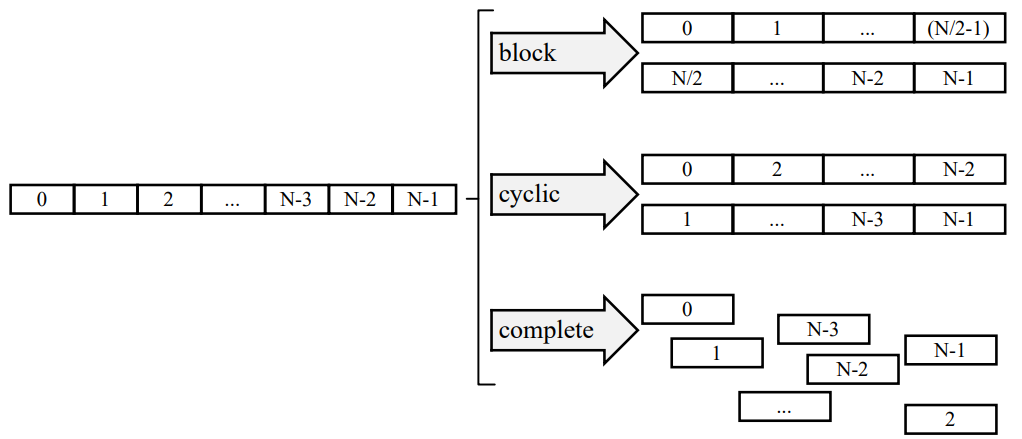
\includegraphics[width=1\textwidth]{introduction/partitioning.png}
	\caption{HLS Array Partitioning}
\end{figure}

	\newpage
	
	\section{Tasks to be performed}
	Prendendo come riferimento il formato CRS per il calcolo del prodotto tra una matrice sparsa ed un vettore e considerando il tool di sintesi ad alto livello per sistemi digitali, fornito da {Xilinx\textsuperscript{\textregistered}, analizzare le soluzioni proposte nella seguente tabella utilizzando le direttive proprietarie citate e caratterizzando in termini di latenza e utilizzazione delle risorse.

\begin{table}[H]
	\centering
	\begin{tabular}{|c|c|c|}
		\hline
		\textbf{Solution} & Loop1 & Loop2 \\
		\hline
		1 & - & - \\
		\hline
		2 & - & Pipeline \\
		\hline
		3 & Pipeline & - \\
		\hline
		4 & Unroll=2 & - \\
		\hline
		5 & - & Pipeline, Unroll=2 \\
		\hline
		6 & - & Pipeline, Unroll=2, Cyclic=2 \\
		\hline
		7 & - & Pipeline, Unroll=4 \\
		\hline
		8 & - & Pipeline, Unroll=2, Cyclic=4 \\
		\hline
		9 & - & Pipeline, Unroll=8 \\
		\hline
		10 & - & Pipeline, Unroll=2, Cyclic=8 \\
		\hline
		11 & - & Pipeline, Unroll=2, Block=8 \\
		\hline
	\end{tabular}
	\caption{SMVM Solutions To Be Performed}
	\label{tab:smvm-solutions-to-be-performed}
\end{table}
	\newpage
	
	\section{Definitions}
	Qui di seguito vengono riportate le definizioni e le intestazioni dei metodi corrispondenti alle soluzioni implementate per la moltiplicazione tra una matrice sparsa e un vettore. In particolare, ogni definizione presenta la documentazione associata. Inoltre, è stata prevista l'implementazione per la moltiplicazione standard così da poter verificare i risultati ottenuti tramite formato CRS.

\lstinputlisting[language=C]{definitions/definitions.h}
	\newpage
	
	\section{C Simulations}
	Qui di seguito viene riportato il file testbench per la C Simulation in HLS e il corrispondente output ottenuto. In particolare, qui di seguito verrà riportato il caso in cui venga scelta la prima configurazione con matrice di dimensione $4*4$. Le altre configurazioni, relative ad alcune solution implementate, verranno presentate nei paragrafi successivi.

\lstinputlisting[language=C++]{c_simulations/smvmTB.cpp}
\lstinputlisting[language=C++]{c_simulations/smvmTB_output.cpp}

Nello specifico, qui di seguito, viene riportata l'implementazione della moltiplicazione standard utilizzata per verificare i risultati sopra allegati.
\lstinputlisting[language=C++]{c_simulations/stdm.cpp}

	\newpage
	
	\section{Solutions}
	Di seguito verranno illustrate e analizzate le soluzioni previste nella tabella sotto allegata. In particolare, nelle implementazioni dove è previsto l'utilizzo della direttiva di partitioning sono stati considerati tre array (columnIndex, values, x) a cui corrispondono quattro solution differenti. Nello specifico, è stata prevista una soluzione in cui viene effettuato il partitioning di tutte e tre gli array contemporaneamente e le rimanenti tre implementazioni in cui, per ognuna di essa, è stato previsto il partizionamento singolo di uno dei tre array appena citati. Tali implementazioni sono riportate qui di seguito.

\begin{table}[H]
	\centering
	\begin{tabular}{|c|c|l|}
		\hline
		\textbf{Solution} & Loop1 & Loop2 \\
		\hline
		1 & - & - \\
		\hline
		2 & - & Pipeline \\
		\hline
		3 & Pipeline & - \\
		\hline
		4 & Unroll=2 & - \\
		\hline
		5 & - & Pipeline, Unroll=2 \\
		\hline
		6 & - & Pipeline, Unroll=2, Cyclic=2 \\
		&\footnotesize{-}&\tabitem{Pipeline, Unroll=2, Cyclic=2 (columnIndex)}\\
		&\footnotesize{-}&\tabitem{Pipeline, Unroll=2, Cyclic=2 (values)}\\
		&\footnotesize{-}&\tabitem{Pipeline, Unroll=2, Cyclic=2 (x)}\\
		&\footnotesize{-}&\tabitem{Pipeline, Unroll=2, Cyclic=2 (columnIndex, values, x)}\\
		\hline
		7 & - & Pipeline, Unroll=4 \\
		\hline
		8 & - & Pipeline, Unroll=2, Cyclic=4 \\
		&\footnotesize{-}&\tabitem{Pipeline, Unroll=2, Cyclic=4 (columnIndex)}\\
		&\footnotesize{-}&\tabitem{Pipeline, Unroll=2, Cyclic=4 (values)}\\
		&\footnotesize{-}&\tabitem{Pipeline, Unroll=2, Cyclic=4 (x)}\\
		&\footnotesize{-}&\tabitem{Pipeline, Unroll=2, Cyclic=4 (columnIndex, values, x)}\\
		\hline
		9 & - & Pipeline, Unroll=8 \\
		\hline
		10 & - & Pipeline, Unroll=2, Cyclic=8 \\
		&\footnotesize{-}&\tabitem{Pipeline, Unroll=2, Cyclic=8 (columnIndex)}\\
		&\footnotesize{-}&\tabitem{Pipeline, Unroll=2, Cyclic=8 (values)}\\
		&\footnotesize{-}&\tabitem{Pipeline, Unroll=2, Cyclic=8 (x)}\\
		&\footnotesize{-}&\tabitem{Pipeline, Unroll=2, Cyclic=8 (columnIndex, values, x)}\\
		\hline
		11 & - & Pipeline, Unroll=2, Block=8 \\
		&\footnotesize{-}&\tabitem{Pipeline, Unroll=2, Block=8 (columnIndex)}\\
		&\footnotesize{-}&\tabitem{Pipeline, Unroll=2, Block=8 (values)}\\
		&\footnotesize{-}&\tabitem{Pipeline, Unroll=2, Block=8 (x)}\\
		&\footnotesize{-}&\tabitem{Pipeline, Unroll=2, Block=8 (columnIndex, values, x)}\\
		\hline
	\end{tabular}
	\caption{Detailed SMVM Solutions To Be Performed}
	\label{tab:detailed-smvm-solutions-to-be-performed}
\end{table}


\newpage

\subsection{Solution 1}
Qui, di seguito, viene riportata l'architettura relativa alla prima solution. 

\lstinputlisting[language=C++]{solutions/s1/s1.cpp}

Si può notare come venga utilizzata una variabile temporanea \textit{ytmp} poiché essa viene utilizzata per calcolare l'uscita corrispondente. In particolare, il risultato calcolato ad ogni iterazione viene sommato a quello della precedente iterazione. Pertanto, essendo che l'uscita deve essere solo assegnata e non letta per ogni iterazione, si utilizza una variabile temporanea per calcolare il risultato. Solo alla fine delle iterazioni si potrà assegnare il risultato all'uscita corrispondente. 

Effettuando la sintesi è possibile evidenziare il seguente report:\\
\begin{table}[H]
	\centering
	\begin{minipage}[t]{0.45\linewidth}
		\centering
		\begin{tabular}{|c|c|c|c|}
			\hline
			\textbf{Clock} & \textbf{Target} & \textbf{Estimated} & \textbf{Uncertainty} \\
			\hline
			ap\_clk & 10.00 & 8.510 & 1.25 \\
			\hline
		\end{tabular}
		\caption{HLS Solution 1 without Trip Count Timing Summary (ns)}
		\label{tab:hls-solution-1-timing-summary}
	\end{minipage}
	\hfill
	\begin{minipage}[t]{0.45\linewidth}
		\centering
		\begin{tabular}{|c|c|c|c|}
			\hline
			\multicolumn{2}{|c|}{\textbf{Latency}} & \multicolumn{2}{|c|}{\textbf{Interval}} \\
			min & max & min & max \\
			\hline
			? & ? & ? & ? \\
			\hline
		\end{tabular}
		\caption{HLS Unoptimized Solution without Trip Count Latency Summary (clock cycles)}
		\label{tab:hls-unoptimized-solution-latency-summary}
	\end{minipage}
\end{table}

\begin{table}[H]
	\centering
	\begin{tabular}{|c|c|c|c|c|c|c|c|c|}
		\hline
		\multicolumn{1}{|c|}{Loop} & \multicolumn{2}{|c|}{\textbf{Latency}} & \multicolumn{2}{c|}{\textbf{Iteration Latency}} & \multicolumn{2}{c|}{\textbf{Initiation Interval}} & \multicolumn{1}{c|}{\textbf{Trip Count}}  \\
		Name & min & max & min & max & achieved & target &  \\
		\hline
		- loop1 & ? & ? & ? & ? & - & - & 4 \\
		+ loop2 & ? & ? & 5 & 5 & - & - & ? \\
		\hline
	\end{tabular}
	\caption{HLS Solution 1 without Trip Count Latency Loops Summary}
	\label{tab:hls-solution-1-loop-summary}
\end{table}

Si può notare come la latenza associata a questa architettura risulta essere "?", cioè non definita. In particolare tale non definizione è dovuta al loop2 del quale non è definito il trip count associato essendo il numero di iterazioni corrispondente non noto a priori. Nello specifico, il ciclo 2 dipende dai valori presenti all'interno dell'array \textit{iFirstEl} che non sono incogniti poiché dipendono dai valori in input all'architettura. Viceversa, la latenza per ogni iterazione (IL), essendo che dipende dalla tipologia di operazioni, risulta essere definita. Per quanto riguarda, invece, il loop1, esso presenta un'iteration latency non definita poiché dipendente direttamente dal loop2 di cui non si è a conoscenza della latenza totale come spiegato precedentemente. Pertanto, la latenza totale del loop1 e, di conseguenza, la latenza totale associata all'architettura risulta essere non nota a priori. Quindi, per poter risolvere si specifica all'interno dell'implementazione la direttiva trip\_count. 

\input{solutions/s1/TripCount}

Pertanto, si allega l'architettura risultante.
\lstinputlisting[language=C++]{solutions/s1/s1tripcount.cpp}

Effettuando la sintesi è possibile evidenziare il seguente report:\\
\begin{table}[H]
	\centering
	\begin{minipage}[t]{0.45\linewidth}
		\centering
		\begin{tabular}{|c|c|c|c|}
			\hline
			\textbf{Clock} & \textbf{Target} & \textbf{Estimated} & \textbf{Uncertainty} \\
			\hline
			ap\_clk & 10.00 & 8.510 & 1.25 \\
			\hline
		\end{tabular}
		\caption{HLS Solution 1 with Trip Count Timing Summary (ns)}
		\label{tab:hls-solution-1-timing-summary}
	\end{minipage}
	\hfill
	\begin{minipage}[t]{0.45\linewidth}
		\centering
		\begin{tabular}{|c|c|c|c|}
			\hline
			\multicolumn{2}{|c|}{\textbf{Latency}} & \multicolumn{2}{|c|}{\textbf{Interval}} \\
			min & max & min & max \\
			\hline
			13 & 93 & 13 & 93 \\
			\hline
		\end{tabular}
		\caption{HLS Unoptimized Solution with Trip Count Latency Summary (clock cycles)}
		\label{tab:hls-unoptimized-solution-latency-summary}
	\end{minipage}
\end{table}

\begin{table}[H]
	\centering
	\begin{tabular}{|c|c|c|c|c|c|c|c|c|}
		\hline
		\multicolumn{1}{|c|}{Loop} & \multicolumn{2}{|c|}{\textbf{Latency}} & \multicolumn{2}{c|}{\textbf{Iteration Latency}} & \multicolumn{2}{c|}{\textbf{Initiation Interval}} & \multicolumn{1}{c|}{\textbf{Trip Count}}  \\
		Name & min & max & min & max & achieved & target &  \\
		\hline
		- loop1 & 12 & 92 & 3 & 23 & - & - & 4 \\
		+ loop2 & 0 & 20 & 5 & 5 & - & - & 0$\sim$4 \\
		\hline
	\end{tabular}
	\caption{HLS Solution 1 Latency with Trip Count Loops Summary }
	\label{tab:hls-solution-1-loop-summary}
\end{table}

Qui di seguito, viene allegato l'utilizzazione delle risorse stimata dal processo di sintesi.
\begin{table}[h]
	\centering
	\begin{tabular}{|l|c|c|c|c|}
		\hline
		\textbf{Name}    & \textbf{BRAM\_18K} & \textbf{DSP48E} & \textbf{FF} & \textbf{LUT} \\ \hline
		DSP              & -                   & -               & -           & -            \\ 
		Expression       & -                   & 3               & 0           & 137          \\ 
		FIFO             & -                   & -               & -           & -            \\ 
		Instance         & -                   & -               & -           & -            \\ 
		Memory           & 0                   & -               & -          & -            \\ 
		Multiplexer      & -                   & -               & -           & 71          \\ 
		Register         & -                   & -               & 241         & -            \\ \hline
		\textbf{Total}   & 0                   & 3               & 241         & 208          \\ \hline
		\textbf{Available} & 280               & 220             & 106400      & 53200        \\ \hline
		\textbf{Utilization (\%)} & 0            & 1               & $\sim$0     & $\sim$0      \\ \hline
	\end{tabular}
	\caption{HLS Solution 1 with Trip Count Utilization Estimates Summary}
	\label{tab:hls-solution-1-utilization-estimates-summary}
\end{table}

Successivamente effettuando la C/RTL Cosimulation e l'Export RTL è possibile evidenziare i seguenti report.
\begin{table}[H]
	\centering
	\begin{tabular}{|c|c|c|c|c|c|c|c|}
		\hline
		\multicolumn{1}{|c|}{RTL} & \multicolumn{1}{|c|}{Status} & \multicolumn{3}{c|}{\textbf{Latency}} & \multicolumn{3}{c|}{\textbf{Interval}} \\
		&  & min & avg & max & min & avg & max \\
		\hline
		VHDL & Pass & 58 & 58 & 58 & 58 & 58 & 58 \\
		\hline
	\end{tabular}
	\caption{HLS Solution 1 with Trip Count C/RTL Cosimulation Summary }
	\label{tab:hls-solution-1-cosimulation-summary}
\end{table}

\begin{table}[H]
	\centering
	\begin{minipage}[t]{0.45\linewidth}
		\centering
		\begin{tabular}{|l|r|}
			\hline
			\textbf{Resource} & \textbf{VHDL} \\
			\hline
			SLICE & 45 \\
			\hline
			LUT & 93 \\
			\hline
			FF & 161 \\
			\hline
			DSP & 3 \\
			\hline
			BRAM & 0 \\
			\hline
			SRL & 0 \\
			\hline
		\end{tabular}
		\caption{HLS Solution 1 with Trip Count Export RTL Resource Usage}
		\label{tab:hls-solution-1-export-rtl-resoruce-usage}
	\end{minipage}
	\hfill
	\begin{minipage}[t]{0.45\linewidth}
		\centering
		\begin{tabular}{|l|r|}
			\hline
			\textbf{Timing} & \textbf{VHDL} \\
			\hline
			CP required & 10.000 \\
			\hline
			CP achieved post-synthesis & 5.745 \\
			\hline
			CP achieved post-implementation & 5.692 \\
			\hline
		\end{tabular}
		\caption{HLS Solution with Trip Count Export RTL Final Timing}
		\label{tab:hls-solution-1-export-rtl-final-timing}
	\end{minipage}
\end{table}
\newpage

\subsection{Solution 2}
Qui, di seguito, viene riportata l'architettura relativa alla seconda solution.

\lstinputlisting[language=C++]{solutions/s2/s2.cpp}

In particolare, nella soluzione hardware in questione, rispetto alla solution 1, è stato aggiunto la direttiva di pipeline all'interno del loop2. Pertanto, ci si dovrebbe aspettare una minore latenza totale dal momento che il pipelining permette di scindere le operazioni complesse in più operazioni semplici. In questo modo si può far lavorare l’architettura con dati temporalmente differenti. 

\begin{figure}[H]
	\centering
	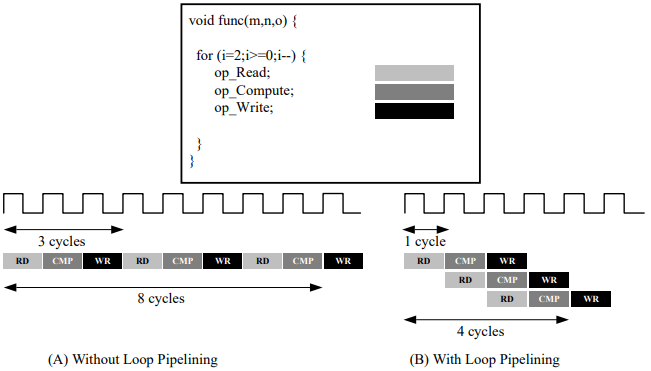
\includegraphics[width=0.5\textwidth]{solutions/s2/looppipelining.png}
	\caption{HLS Loop Pipelining}
\end{figure}

Effettuando la sintesi è possibile evidenziare il seguente report:\\

\begin{table}[H]
	\centering
	\begin{minipage}[t]{0.45\linewidth}
		\centering
		\begin{tabular}{|c|c|c|c|}
			\hline
			\textbf{Clock} & \textbf{Target} & \textbf{Estimated} & \textbf{Uncertainty} \\
			\hline
			ap\_clk & 10.00 & 8.510 & 1.25 \\
			\hline
		\end{tabular}
		\caption{HLS Solution 2 Timing Summary (ns)}
		\label{tab:hls-solution-2-timing-summary}
	\end{minipage}
	\hfill
	\begin{minipage}[t]{0.45\linewidth}
		\centering
		\begin{tabular}{|c|c|c|c|}
			\hline
			\multicolumn{2}{|c|}{\textbf{Latency}} & \multicolumn{2}{|c|}{\textbf{Interval}} \\
			min & max & min & max \\
			\hline
			17 & 45 & 17 & 45 \\
			\hline
		\end{tabular}
		\caption{HLS Solution 2 Latency Summary (clock cycles)}
		\label{tab:hls-solution-2-latency-summary}
	\end{minipage}
\end{table}

\begin{table}[H]
	\centering
	\begin{tabular}{|c|c|c|c|c|c|c|c|c|}
		\hline
		\multicolumn{1}{|c|}{Loop} & \multicolumn{2}{|c|}{\textbf{Latency}} & \multicolumn{1}{c|}{\textbf{Iteration Latency}} & \multicolumn{2}{c|}{\textbf{Initiation Interval}} & \multicolumn{1}{c|}{\textbf{Trip Count}}  \\
		Name & min & max &  & achieved & target &  \\
		\hline
		- loop1 & 16 & 44 & 4$\sim$11 & - & - & 4 \\
		+ loop2 & 0 & 7 & 5 & 1 & 1 & 0$\sim$4 \\
		\hline
	\end{tabular}
	\caption{HLS Solution 2 Latency Loops Summary}
	\label{tab:hls-solution-2-loop-summary}
\end{table}

Si può notare, rispetto alla solution precedente, come in questo caso venga specificato un valore numerico di Initiation Interval (II). In particolare, l'II\_achieved risulta essere il medesimo di quello target, cioè uguale a 1. Teoricamente, come in questo caso, si dovrebbe ottenere II\_target=II\_achieved. Se così non fosse allora il tool non è riuscito a raggiungere l'obiettivo prefissato e si dovrebbero attuare modifiche all'architetture o caso mai prevedere l'utilizzo di ulteriori direttive.
\\
Qui di seguito, viene allegato l'utilizzazione delle risorse stimata dal processo di sintesi.
\begin{table}[H]
	\centering
	\begin{tabular}{|l|c|c|c|c|}
		\hline
		\textbf{Name}    & \textbf{BRAM\_18K} & \textbf{DSP48E} & \textbf{FF} & \textbf{LUT} \\ \hline
		DSP              & -                   & -               & -           & -            \\ 
		Expression       & -                   & 3               & 0           & 141          \\ 
		FIFO             & -                   & -               & -           & -            \\ 
		Instance         & -                   & -               & -           & -            \\ 
		Memory           & 0                   & -               & -          & -            \\ 
		Multiplexer      & -                   & -               & -           & 78          \\ 
		Register         & -                   & -               & 340         & 32            \\ \hline
		\textbf{Total}   & 0                   & 3               & 340         & 251          \\ \hline
		\textbf{Available} & 280               & 220             & 106400      & 53200        \\ \hline
		\textbf{Utilization (\%)} & 0            & 1               & $\sim$0     & $\sim$0      \\ \hline
	\end{tabular}
	\caption{HLS Solution 2 Utilization Estimates Summary}
	\label{tab:hls-solution-2-utilization-estimates-summary}
\end{table}

Successivamente effettuando la C/RTL Cosimulation e l'Export RTL è possibile evidenziare i seguenti report.
\begin{table}[H]
	\centering
	\begin{tabular}{|c|c|c|c|c|c|c|c|}
		\hline
		\multicolumn{1}{|c|}{RTL} & \multicolumn{1}{|c|}{Status} & \multicolumn{3}{c|}{\textbf{Latency}} & \multicolumn{3}{c|}{\textbf{Interval}} \\
		&  & min & avg & max & min & avg & max \\
		\hline
		VHDL & Pass & 38 & 38 & 38 & NA & NA & NA \\
		\hline
	\end{tabular}
	\caption{HLS Solution 1 with Trip Count C/RTL Cosimulation Summary }
	\label{tab:hls-solution-1-cosimulation-summary}
\end{table}

In particolare, si può notare come, in seguito all'introduzione della direttiva di pipeline, il numero di risorse risulta essere cambiato. Nello specifico, l'utilizzazione delle LUT è aumentata di circa il $24\%$ mentre quella dei FF è diminuita di circa il $14\%$.

\begin{table}[H]
	\centering
	\begin{minipage}[t]{0.45\linewidth}
		\centering
		\begin{tabular}{|l|r|}
			\hline
			\textbf{Resource} & \textbf{VHDL} \\
			\hline
			SLICE & 38 \\
			\hline
			LUT & 115 \\
			\hline
			FF & 139 \\
			\hline
			DSP & 3 \\
			\hline
			BRAM & 0 \\
			\hline
			SRL & 0 \\
			\hline
		\end{tabular}
		\caption{HLS Solution 2t Export RTL Resource Usage}
		\label{tab:hls-solution-2-export-rtl-resoruce-usage}
	\end{minipage}
	\hfill
	\begin{minipage}[t]{0.45\linewidth}
		\centering
		\begin{tabular}{|l|r|}
			\hline
			\textbf{Timing} & \textbf{VHDL} \\
			\hline
			CP required & 10.000 \\
			\hline
			CP achieved post-synthesis & 5.745 \\
			\hline
			CP achieved post-implementation & 5.718 \\
			\hline
		\end{tabular}
		\caption{HLS Solution 2 Export RTL Final Timing}
		\label{tab:hls-solution-2-export-rtl-final-timing}
	\end{minipage}
\end{table}
\newpage

\subsection{Solution 3}
Qui, di seguito, viene riportata l'architettura relativa alla terza solution.

\lstinputlisting[language=C++]{solutions/s3/s3.cpp}

In particolare, nella soluzione hardware in questione, rispetto alla solution 1, è stato aggiunta la direttiva di pipeline all'interno del loop1.

Effettuando la sintesi è possibile evidenziare il seguente report:\\

\begin{table}[H]
	\centering
	\begin{minipage}[t]{0.45\linewidth}
		\centering
		\begin{tabular}{|c|c|c|c|}
			\hline
			\textbf{Clock} & \textbf{Target} & \textbf{Estimated} & \textbf{Uncertainty} \\
			\hline
			ap\_clk & 10.00 & 8.510 & 1.25 \\
			\hline
		\end{tabular}
		\caption{HLS Solution 3 Timing Summary (ns)}
		\label{tab:hls-solution-3-timing-summary}
	\end{minipage}
	\hfill
	\begin{minipage}[t]{0.45\linewidth}
		\centering
		\begin{tabular}{|c|c|c|c|}
			\hline
			\multicolumn{2}{|c|}{\textbf{Latency}} & \multicolumn{2}{|c|}{\textbf{Interval}} \\
			min & max & min & max \\
			\hline
			13 & 93 & 13 & 93 \\
			\hline
		\end{tabular}
		\caption{HLS Solution 3 Latency Summary (clock cycles)}
		\label{tab:hls-solution-3-latency-summary}
	\end{minipage}
\end{table}

\begin{table}[H]
	\centering
	\begin{tabular}{|c|c|c|c|c|c|c|c|c|}
		\hline
		\multicolumn{1}{|c|}{Loop} & \multicolumn{2}{|c|}{\textbf{Latency}} & \multicolumn{1}{c|}{\textbf{Iteration Latency}} & \multicolumn{2}{c|}{\textbf{Initiation Interval}} & \multicolumn{1}{c|}{\textbf{Trip Count}}  \\
		Name & min & max &  & achieved & target &  \\
		\hline
		- loop1 & 12 & 92 & 3$\sim$23 & - & - & 4 \\
		+ loop2 & 0 & 20 & 5 & - & - & 0$\sim$4 \\
		\hline
	\end{tabular}
	\caption{HLS Solution 3 Latency Loops Summary}
	\label{tab:hls-solution-3-loop-summary}
\end{table}

Si può notare come, in questo caso l'Initiation Interval sia non specificato nel loop2 dal momento che la direttiva introdotta nella solution 2 è stata eliminata per la soluzione hardware in questione. Molto più importante è che, considerando la direttiva di pipeline definita all'interno del loop1, in corrispondenza dell'Initiation Interval di tale ciclo non è definito alcun valore numerico. Tanto è vero che, analizzando i log della sintesi presenti nella console è possibile identificare il seguente warning.
\\
WARNING: [SCHED 204-65] Unable to satisfy pipeline directive: Loop contains subloop(s) not being unrolled or flattened.
\\
In particolare, è come se il tool non riuscisse a soddisfare la richiesta di pipeline per il loop1 effettuata tramite la direttiva proprietaria. Questo potrebbe essere giustificato dal fatto che effettivamente la scissione dell'operazione "complessa" in micro-operazioni, all'interno del ciclo in questione, non è possibile effettuarla. Infatti, si può notare come i valori di latenza siano i medesimi di quelli della solution 1. Effettivamente, si potrebbe aggiungere la direttiva di pipeline all'interno del loop2, come fatto per la solution 2, dove sono presenti la maggior parte delle operazioni. In quel caso, infatti, il tool è riuscito a scomporre in micro-operazioni e così da permettere una minore latenza dal momento che i moduli potevano essere utilizzati da dati temporalmente differenti. Quello che si può notare è che nel loop1 le operazioni risultano essere l'inizializzazione della variabile temporanea \textit{ytmp}, le operazioni interne al loop2 e la scrittura del valore di \textit{ytmp} in \textit{y}. Pertanto, le uniche operazioni complesse che potrebbero essere gestite tramite una direttiva di pipeline si trovano all'interno del loop2.

\begin{figure}[H]
	\centering
	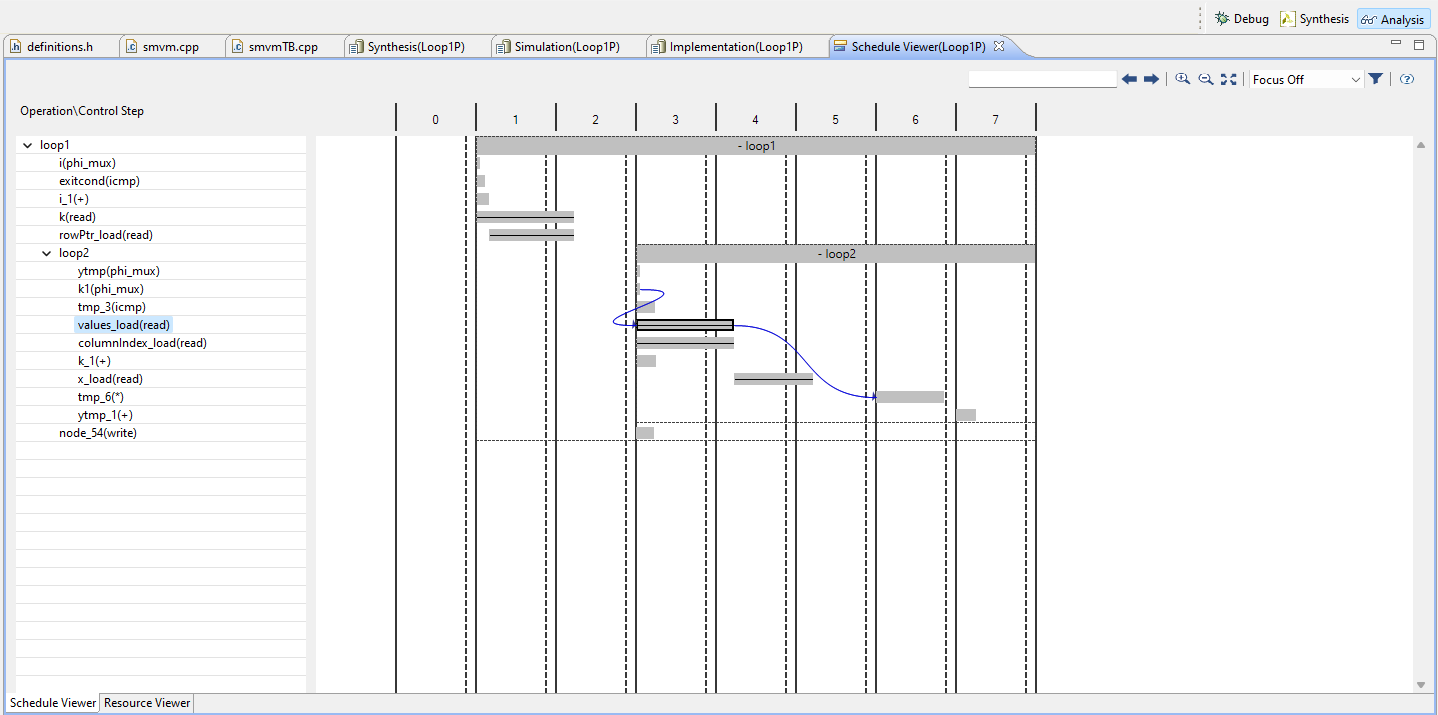
\includegraphics[width=1\textwidth]{solutions/s3/loop1pipeline.png}
	\caption{HLS Solution 3 Analysis}
\end{figure}

Qui di seguito, viene allegato l'utilizzazione delle risorse stimata dal processo di sintesi. Anche in questo caso il numero di risorse è il medesimo di quello ottenuto in corrispondenza della solution 1.
\begin{table}[h]
	\centering
	\begin{tabular}{|l|c|c|c|c|}
		\hline
		\textbf{Name}    & \textbf{BRAM\_18K} & \textbf{DSP48E} & \textbf{FF} & \textbf{LUT} \\ \hline
		DSP              & -                   & -               & -           & -            \\ 
		Expression       & -                   & 3               & 0           & 137          \\ 
		FIFO             & -                   & -               & -           & -            \\ 
		Instance         & -                   & -               & -           & -            \\ 
		Memory           & 0                   & -               & -          & -            \\ 
		Multiplexer      & -                   & -               & -           & 71          \\ 
		Register         & -                   & -               & 241         & -            \\ \hline
		\textbf{Total}   & 0                   & 3               & 241         & 208          \\ \hline
		\textbf{Available} & 280               & 220             & 106400      & 53200        \\ \hline
		\textbf{Utilization (\%)} & 0            & 1               & $\sim$0     & $\sim$0      \\ \hline
	\end{tabular}
	\caption{HLS Solution 3 Utilization Estimates Summary}
	\label{tab:hls-solution-3-utilization-estimates-summary}
\end{table}

Successivamente effettuando la C/RTL Cosimulation e l'Export RTL è possibile evidenziare i seguenti report. Anche in questo caso, sia il report del C/RTL Cosimulation sia quello dell'Export RTL risultano essere i medesimi di quelli della solution 1.
\begin{table}[H]
	\centering
	\begin{tabular}{|c|c|c|c|c|c|c|c|}
		\hline
		\multicolumn{1}{|c|}{RTL} & \multicolumn{1}{|c|}{Status} & \multicolumn{3}{c|}{\textbf{Latency}} & \multicolumn{3}{c|}{\textbf{Interval}} \\
		&  & min & avg & max & min & avg & max \\
		\hline
		VHDL & Pass & 58 & 58 & 58 & NA & NA & NA \\
		\hline
	\end{tabular}
	\caption{HLS Solution 1 with Trip Count C/RTL Cosimulation Summary }
	\label{tab:hls-solution-1-cosimulation-summary}
\end{table}

\begin{table}[H]
	\centering
	\begin{minipage}[t]{0.45\linewidth}
		\centering
		\begin{tabular}{|l|r|}
			\hline
			\textbf{Resource} & \textbf{VHDL} \\
			\hline
			SLICE & 48 \\
			\hline
			LUT & 94 \\
			\hline
			FF & 161 \\
			\hline
			DSP & 3 \\
			\hline
			BRAM & 0 \\
			\hline
			SRL & 0 \\
			\hline
		\end{tabular}
		\caption{HLS Solution 2t Export RTL Resource Usage}
		\label{tab:hls-solution-2-export-rtl-resoruce-usage}
	\end{minipage}
	\hfill
	\begin{minipage}[t]{0.45\linewidth}
		\centering
		\begin{tabular}{|l|r|}
			\hline
			\textbf{Timing} & \textbf{VHDL} \\
			\hline
			CP required & 10.000 \\
			\hline
			CP achieved post-synthesis & 5.745 \\
			\hline
			CP achieved post-implementation & 5.692 \\
			\hline
		\end{tabular}
		\caption{HLS Solution 2 Export RTL Final Timing}
		\label{tab:hls-solution-2-export-rtl-final-timing}
	\end{minipage}
\end{table}


Pertanto, considerando la solution in questione, la si potrebbe modificare aggiungendo la direttiva di pipeline anche nel loop2 per capire se le ipotesi, effettuate precedentemente, possono essere confermate o meno. 

\lstinputlisting[language=C++]{solutions/s3/s3modificata.cpp}

Adottando questo approccio, però, la nuova soluzione hardware in questione si ricondurrebbe alla solution 2 precedentemente analizzata dal momento che la direttiva di pipeline nel loop1 verrebbe comunque ignorata e quello che verrebbe effettivamente attuato sarebbe il pragma di pipeline all'interno del loop2. Infatti, effettuando la sintesi si può notare come sia presente il medeesimo warning, alleegato precedentemente, e come sia i valori di latenza sia quelli dell'utilizzazione delle risorse siano i medesimi.
\\
WARNING: [SCHED 204-65] Unable to satisfy pipeline directive: Loop contains subloop(s) not being unrolled or flattened.

\begin{table}[H]
	\centering
	\begin{minipage}[t]{0.45\linewidth}
		\centering
		\begin{tabular}{|c|c|c|c|}
			\hline
			\textbf{Clock} & \textbf{Target} & \textbf{Estimated} & \textbf{Uncertainty} \\
			\hline
			ap\_clk & 10.00 & 8.510 & 1.25 \\
			\hline
		\end{tabular}
		\caption{HLS Solution 3 Modified Timing Summary (ns)}
		\label{tab:hls-solution-3-modified-timing-summary}
	\end{minipage}
	\hfill
	\begin{minipage}[t]{0.45\linewidth}
		\centering
		\begin{tabular}{|c|c|c|c|}
			\hline
			\multicolumn{2}{|c|}{\textbf{Latency}} & \multicolumn{2}{|c|}{\textbf{Interval}} \\
			min & max & min & max \\
			\hline
			17 & 45 & 17 & 45 \\
			\hline
		\end{tabular}
		\caption{HLS Solution 3 Modified Latency Summary (clock cycles)}
		\label{tab:hls-solution-3-modified-latency-summary}
	\end{minipage}
\end{table}

\begin{table}[H]
	\centering
	\begin{tabular}{|c|c|c|c|c|c|c|c|c|}
		\hline
		\multicolumn{1}{|c|}{Loop} & \multicolumn{2}{|c|}{\textbf{Latency}} & \multicolumn{1}{c|}{\textbf{Iteration Latency}} & \multicolumn{2}{c|}{\textbf{Initiation Interval}} & \multicolumn{1}{c|}{\textbf{Trip Count}}  \\
		Name & min & max &  & achieved & target &  \\
		\hline
		- loop1 & 16 & 44 & 4$\sim$11 & - & - & 4 \\
		+ loop2 & 0 & 7 & 5 & 1 & 1 & 0$\sim$4 \\
		\hline
	\end{tabular}
	\caption{HLS Solution 3 Modified Latency Loops Summary}
	\label{tab:hls-solution-3-modified-loop-summary}
\end{table}

\begin{table}[h]
	\centering
	\begin{tabular}{|l|c|c|c|c|}
		\hline
		\textbf{Name}    & \textbf{BRAM\_18K} & \textbf{DSP48E} & \textbf{FF} & \textbf{LUT} \\ \hline
		DSP              & -                   & -               & -           & -            \\ 
		Expression       & -                   & 3               & 0           & 141          \\ 
		FIFO             & -                   & -               & -           & -            \\ 
		Instance         & -                   & -               & -           & -            \\ 
		Memory           & 0                   & -               & -          & -            \\ 
		Multiplexer      & -                   & -               & -           & 78          \\ 
		Register         & -                   & -               & 340         & 32            \\ \hline
		\textbf{Total}   & 0                   & 3               & 340         & 251          \\ \hline
		\textbf{Available} & 280               & 220             & 106400      & 53200        \\ \hline
		\textbf{Utilization (\%)} & 0            & 1               & $\sim$0     & $\sim$0      \\ \hline
	\end{tabular}
	\caption{HLS Solution 3 Modified Utilization Estimates Summary}
	\label{tab:hls-solution-3-modified-utilization-estimates-summary}
\end{table}


\newpage

\subsection{Solution 4}
Qui, di seguito, viene riportata l'architettura relativa alla quarta solution.

\lstinputlisting[language=C++]{solutions/s4/s4.cpp}

In particolare, nella soluzione hardware in questione, rispetto alla solution 1, è stata aggiunta la direttiva di unrolling con fattore pari a 2 all'interno del loop1.

\begin{figure}[H]
	\centering
	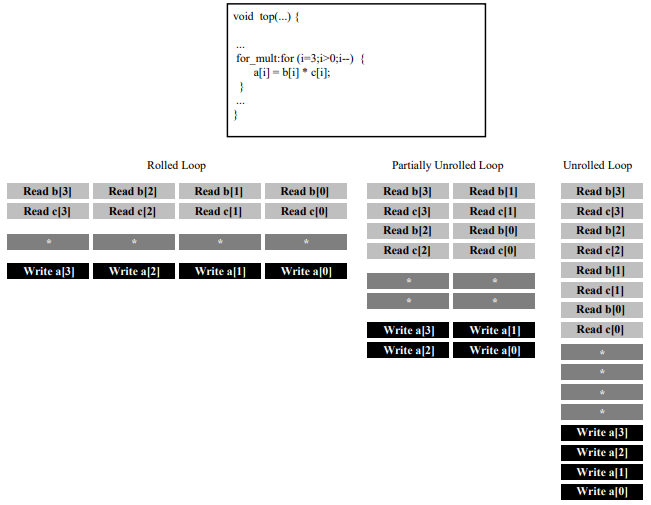
\includegraphics[width=0.5\textwidth]{solutions/s4/unrolling.png}
	\caption{HLS Loop Unrolling}
\end{figure}

Effettuando la sintesi è possibile evidenziare il seguente report:\\

\begin{table}[H]
	\centering
	\begin{minipage}[t]{0.45\linewidth}
		\centering
		\begin{tabular}{|c|c|c|c|}
			\hline
			\textbf{Clock} & \textbf{Target} & \textbf{Estimated} & \textbf{Uncertainty} \\
			\hline
			ap\_clk & 10.00 & 8.510 & 1.25 \\
			\hline
		\end{tabular}
		\caption{HLS Solution 4 Timing Summary (ns)}
		\label{tab:hls-solution-4-timing-summary}
	\end{minipage}
	\hfill
	\begin{minipage}[t]{0.45\linewidth}
		\centering
		\begin{tabular}{|c|c|c|c|}
			\hline
			\multicolumn{2}{|c|}{\textbf{Latency}} & \multicolumn{2}{|c|}{\textbf{Interval}} \\
			min & max & min & max \\
			\hline
			11 & 91 & 11 & 91 \\
			\hline
		\end{tabular}
		\caption{HLS Solution 4 Latency Summary (clock cycles)}
		\label{tab:hls-solution-4-latency-summary}
	\end{minipage}
\end{table}

In particolare, si può notare come il valore di trip count del loop1 risulta essere dimezzato rispetto alla solution 1. Questo è dovuto all'attuazione della direttiva  di unrolling di fattore 2 sul loop1 e così permettendo l'esecuzione in parallelo di due iterazioni.

\begin{table}[H]
	\centering
	\begin{tabular}{|c|c|c|c|c|c|c|c|c|}
		\hline
		\multicolumn{1}{|c|}{Loop} & \multicolumn{2}{|c|}{\textbf{Latency}} & \multicolumn{1}{c|}{\textbf{Iteration Latency}} & \multicolumn{2}{c|}{\textbf{Initiation Interval}} & \multicolumn{1}{c|}{\textbf{Trip Count}}  \\
		Name & min & max &  & achieved & target &  \\
		\hline
		- loop1 & 10 & 90 & 5$\sim$45 & - & - & 2 \\
		+ loop2 & 0 & 20 & 5 & - & - & 0$\sim$4 \\
		+ loop2 & 0 & 20 & 5 & - & - & 0$\sim$4 \\
		\hline
	\end{tabular}
	\caption{HLS Solution 4 Latency Loops Summary}
	\label{tab:hls-solution-4-loop-summary}
\end{table}

Infatti, lo si può meglio notare tramite l'interfaccia analysis. In particolare, si può evidenziare come il loop1 venga parallelizzato. Nello specifico, vengono previsti due loop2 uno dopo l'altro facendo così aumentare la latenza per ogni iterazione del loop1. Quindi, il valore del trip count associato al ciclo 1 viene dimezzato mentre l'Iteration Latency associata allo stesso loop aumenta dal momento che vengono gestiti due loop2.

\begin{figure}[H]
	\centering
	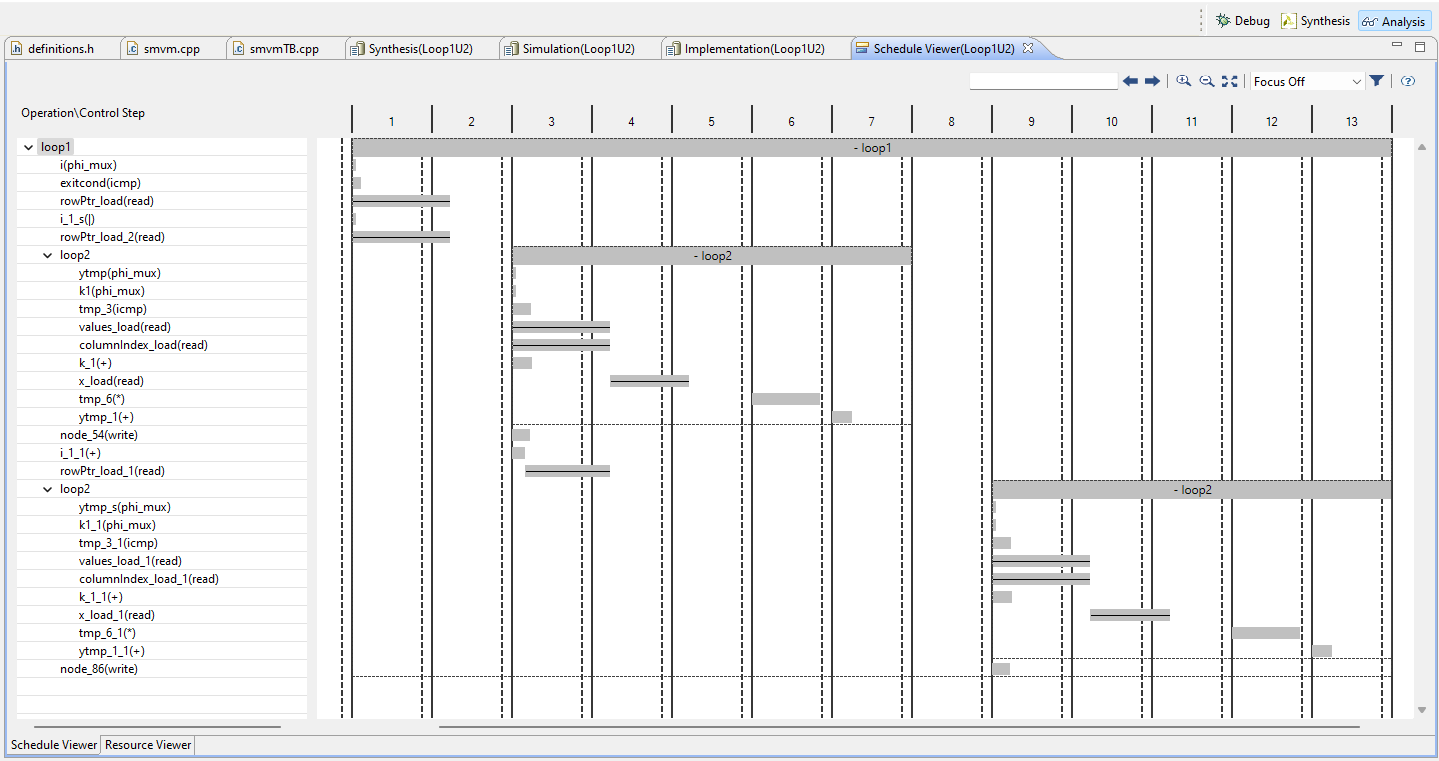
\includegraphics[width=1\textwidth]{solutions/s4/s4analysis.png}
	\caption{HLS Solution 4 Analysis}
\end{figure}

\begin{table}[H]
	\centering
	\begin{tabular}{|l|c|c|c|c|}
		\hline
		\textbf{Name}    & \textbf{BRAM\_18K} & \textbf{DSP48E} & \textbf{FF} & \textbf{LUT} \\ \hline
		DSP              & -                   & -               & -           & -            \\ 
		Expression       & -                   & 3               & 0           & 235          \\ 
		FIFO             & -                   & -               & -           & -            \\ 
		Instance         & -                   & -               & -           & -            \\ 
		Memory           & 0                   & -               & -          & -            \\ 
		Multiplexer      & -                   & -               & -           & 197          \\ 
		Register         & -                   & -               & 376         & -            \\ \hline
		\textbf{Total}   & 0                   & 3               & 376         & 432          \\ \hline
		\textbf{Available} & 280               & 220             & 106400      & 53200        \\ \hline
		\textbf{Utilization (\%)} & 0            & 1               & $\sim$0     & $\sim$0      \\ \hline
	\end{tabular}
	\caption{HLS Solution 4 Utilization Estimates Summary}
	\label{tab:hls-solution-4-utilization-estimates-summary}
\end{table}

Successivamente effettuando la C/RTL Cosimulation e l'Export RTL è possibile evidenziare i seguenti report.

\begin{table}[H]
	\centering
	\begin{tabular}{|c|c|c|c|c|c|c|c|}
		\hline
		\multicolumn{1}{|c|}{RTL} & \multicolumn{1}{|c|}{Status} & \multicolumn{3}{c|}{\textbf{Latency}} & \multicolumn{3}{c|}{\textbf{Interval}} \\
		&  & min & avg & max & min & avg & max \\
		\hline
		VHDL & Pass & 56 & 56 & 56 & NA & NA & NA \\
		\hline
	\end{tabular}
	\caption{HLS Solution 4 C/RTL Cosimulation Summary }
	\label{tab:hls-solution-4-cosimulation-summary}
\end{table}

In particolare, rispetto alla solution 1 si ha un aumento di circa il $73\%$ delle slice, del $100\%$ delle LUT e di circa l'$81\%$ dei FF dal momento che è stato introdotto un parallelismo all'interno dell'architettura.

\begin{table}[H]
	\centering
	\begin{minipage}[t]{0.45\linewidth}
		\centering
		\begin{tabular}{|l|r|}
			\hline
			\textbf{Resource} & \textbf{VHDL} \\
			\hline
			SLICE & 83 \\
			\hline
			LUT & 186 \\
			\hline
			FF & 292 \\
			\hline
			DSP & 3 \\
			\hline
			BRAM & 0 \\
			\hline
			SRL & 0 \\
			\hline
		\end{tabular}
		\caption{HLS Solution 4 Export RTL Resource Usage}
		\label{tab:hls-solution-4-export-rtl-resoruce-usage}
	\end{minipage}
	\hfill
	\begin{minipage}[t]{0.45\linewidth}
		\centering
		\begin{tabular}{|l|r|}
			\hline
			\textbf{Timing} & \textbf{VHDL} \\
			\hline
			CP required & 10.000 \\
			\hline
			CP achieved post-synthesis & 5.745 \\
			\hline
			CP achieved post-implementation & 5.692 \\
			\hline
		\end{tabular}
		\caption{HLS Solution 4 Export RTL Final Timing}
		\label{tab:hls-solution-4-export-rtl-final-timing}
	\end{minipage}
\end{table}
\newpage

\subsection{Solution 5}
Qui, di seguito, viene riportata l'architettura relativa alla quinta solution.

\lstinputlisting[language=C++]{solutions/s5/s5.cpp}

In particolare, nella soluzione hardware in questione, rispetto alla solution 2 dove era presenta solo la direttiva di unrolling nel loop2,, è stata aggiunta la direttiva di unrolling con fattore pari a 2 all'interno del loop2.

Effettuando la sintesi è possibile evidenziare il seguente report:\\

\begin{table}[H]
	\centering
	\begin{minipage}[t]{0.45\linewidth}
		\centering
		\begin{tabular}{|c|c|c|c|}
			\hline
			\textbf{Clock} & \textbf{Target} & \textbf{Estimated} & \textbf{Uncertainty} \\
			\hline
			ap\_clk & 10.00 & 8.510 & 1.25 \\
			\hline
		\end{tabular}
		\caption{HLS Solution 5 Timing Summary (ns)}
		\label{tab:hls-solution-5-timing-summary}
	\end{minipage}
	\hfill
	\begin{minipage}[t]{0.45\linewidth}
		\centering
		\begin{tabular}{|c|c|c|c|}
			\hline
			\multicolumn{2}{|c|}{\textbf{Latency}} & \multicolumn{2}{|c|}{\textbf{Interval}} \\
			min & max & min & max \\
			\hline
			33 & 41 & 33 & 41 \\
			\hline
		\end{tabular}
		\caption{HLS Solution 5 Latency Summary (clock cycles)}
		\label{tab:hls-solution-5-latency-summary}
	\end{minipage}
\end{table}

In particolare, si può notare come, rispetto alla solution 2 dove il trip count relativo al loop2 era pari a $0\sim4$, in questo caso il trip count associato al loop2 risulta essere dimezzato dal momento che è stato previsto un unrolling di fattore pari a 2 all'interno del ciclo in questione. Inoltre, dal momento che è stato introdotto una direttiva di pipeline all'interno del loop2, si può evidenziare come l'Initiation Interval raggiunto risulta essere il medesimo di quello target.

\begin{table}[H]
	\centering
	\begin{tabular}{|c|c|c|c|c|c|c|c|c|}
		\hline
		\multicolumn{1}{|c|}{Loop} & \multicolumn{2}{|c|}{\textbf{Latency}} & \multicolumn{1}{c|}{\textbf{Iteration Latency}} & \multicolumn{2}{c|}{\textbf{Initiation Interval}} & \multicolumn{1}{c|}{\textbf{Trip Count}}  \\
		Name & min & max &  & achieved & target &  \\
		\hline
		- loop1 & 32 & 40 & 8$\sim$10 & - & - & 4 \\
		+ loop2 & 4 & 6 & 5 & 1 & 1 & 0$\sim$2 \\
		\hline
	\end{tabular}
	\caption{HLS Solution 5 Latency Loops Summary}
	\label{tab:hls-solution-5-loop-summary}
\end{table}

Si può notare come, all'interno del loop2, vengono effettuate in parallelo due letture relative alle variabili \textit{columnIndex}, due relative alle variabili \textit{values} e due relative alle variabili \textit{x}. 

\begin{figure}[H]
	\centering
	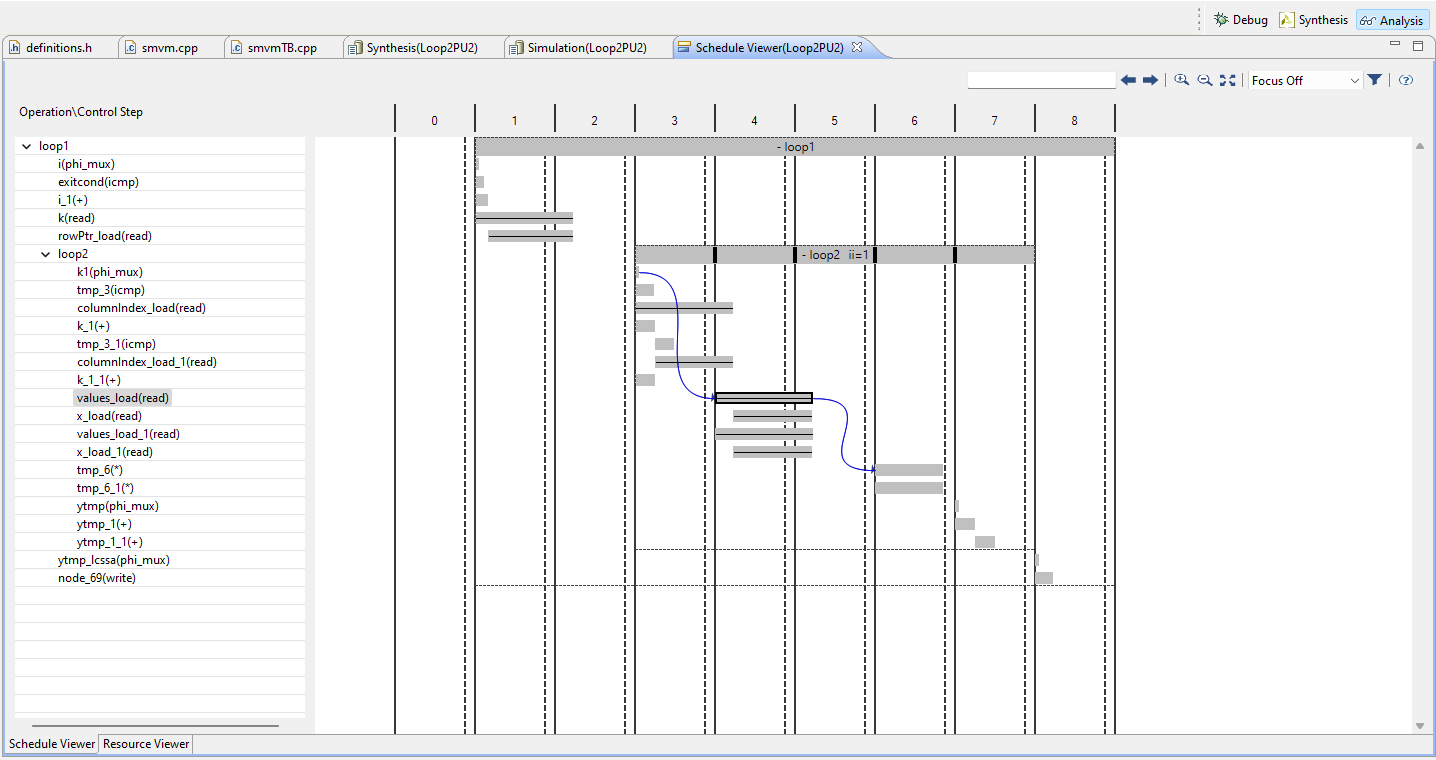
\includegraphics[width=1\textwidth]{solutions/s5/s5analysis.png}
	\caption{HLS Solution 5 Analysis}
\end{figure}

\begin{table}[h]
	\centering
	\begin{tabular}{|l|c|c|c|c|}
		\hline
		\textbf{Name}    & \textbf{BRAM\_18K} & \textbf{DSP48E} & \textbf{FF} & \textbf{LUT} \\ \hline
		DSP              & -                   & -               & -           & -            \\ 
		Expression       & -                   & 6              & 0           & 257          \\ 
		FIFO             & -                   & -               & -           & -            \\ 
		Instance         & -                   & -               & -           & -            \\ 
		Memory           & 0                   & -               & -          & -            \\ 
		Multiplexer      & -                   & -               & -           & 78          \\ 
		Register         & -                   & -               & 597         & 64            \\ \hline
		\textbf{Total}   & 0                   & 6               & 597         & 399          \\ \hline
		\textbf{Available} & 280               & 220             & 106400      & 53200        \\ \hline
		\textbf{Utilization (\%)} & 0            & 2               & $\sim$0     & $\sim$0      \\ \hline
	\end{tabular}
	\caption{HLS Solution 5 Utilization Estimates Summary}
	\label{tab:hls-solution-5-utilization-estimates-summary}
\end{table}

\begin{table}[H]
	\centering
	\begin{tabular}{|c|c|c|c|c|c|c|c|}
		\hline
		\multicolumn{1}{|c|}{RTL} & \multicolumn{1}{|c|}{Status} & \multicolumn{3}{c|}{\textbf{Latency}} & \multicolumn{3}{c|}{\textbf{Interval}} \\
		&  & min & avg & max & min & avg & max \\
		\hline
		VHDL & Pass & 37 & 37 & 37 & NA & NA & NA \\
		\hline
	\end{tabular}
	\caption{HLS Solution 1 with Trip Count C/RTL Cosimulation Summary }
	\label{tab:hls-solution-1-cosimulation-summary}
\end{table}

Si può notare, rispetto alla soluzione hardware 2, un aumento dell'utilizzazione delle risorse del $60\%$ per quanto riguarda le LUT e di circa il $41\%$ per quanto riguarda i FF. Inoltre, si può evidenziare come il numero dei DSP sia raddoppiato.

\begin{table}[H]
	\centering
	\begin{minipage}[t]{0.45\linewidth}
		\centering
		\begin{tabular}{|l|r|}
			\hline
			\textbf{Resource} & \textbf{VHDL} \\
			\hline
			SLICE & 69 \\
			\hline
			LUT & 184 \\
			\hline
			FF & 196 \\
			\hline
			DSP & 6 \\
			\hline
			BRAM & 0 \\
			\hline
			SRL & 0 \\
			\hline
		\end{tabular}
		\caption{HLS Solution 5 Export RTL Resource Usage}
		\label{tab:hls-solution-4-export-rtl-resoruce-usage}
	\end{minipage}
	\hfill
	\begin{minipage}[t]{0.45\linewidth}
		\centering
		\begin{tabular}{|l|r|}
			\hline
			\textbf{Timing} & \textbf{VHDL} \\
			\hline
			CP required & 10.000 \\
			\hline
			CP achieved post-synthesis & 7.927 \\
			\hline
			CP achieved post-implementation & 7.465 \\
			\hline
		\end{tabular}
		\caption{HLS Solution 5 Export RTL Final Timing}
		\label{tab:hls-solution-4-export-rtl-final-timing}
	\end{minipage}
\end{table}
\newpage

\subsection{Solution 6}
Qui, di seguito, vengono riportate le architetture relative alla sesta solution. In particolare, come già precedentemente citato, tale solution prevede l'utilizzo della direttiva di partitioning. Nello specifico, verranno analizzate le seguenti implementazioni relative al loop2:
\begin{itemize}
	\item Pipeline, Unroll=2, Cyclic=2 (columnIndex, values, x)
	\item Pipeline, Unroll=2, Cyclic=2 (columnIndex)
	\item Pipeline, Unroll=2, Cyclic=2 (values)
	\item Pipeline, Unroll=2, Cyclic=2 (x)
\end{itemize}

In particolare, è possibile evidenziare nel dettaglio le differenti soluzioni hardware nei seguenti allegati.
\lstinputlisting[language=C++]{solutions/s6/s6all3.cpp}
\lstinputlisting[language=C++]{solutions/s6/s6columnIndex.cpp}
\lstinputlisting[language=C++]{solutions/s6/s6values.cpp}
\lstinputlisting[language=C++]{solutions/s6/s6x.cpp}

Effettuando la sintesi è possibile evidenziare il seguente report:\\

\begin{table}[H]
	\centering
	\begin{tabular}{|c|c|c|c|c|}
		\hline
		\textbf{Solution} & \textbf{Clock} & \textbf{Target} & \textbf{Estimated} & \textbf{Uncertainty} \\
		\hline
		columnIndex, values, x & ap\_clk & 10.00 & 8.510 & 1.25 \\
		\hline
		columnIndex & ap\_clk & 10.00 & 8.510 & 1.25 \\
		\hline
		values & ap\_clk & 10.00 & 8.510 & 1.25 \\
		\hline
		x & ap\_clk & 10.00 & 8.510 & 1.25 \\
		\hline
	\end{tabular}
	\caption{HLS Solution 6 Timing Summary (ns)}
	\label{tab:hls-solution-6-timing-summary}
\end{table}

\begin{table}[H]
	\centering
	\begin{tabular}{|c|c|c|c|c|}
		\hline
		\multicolumn{1}{|c|}{\textbf{Solution}} & \multicolumn{2}{|c|}{\textbf{Latency}} & \multicolumn{2}{|c|}{\textbf{Interval}} \\
		& min & max & min & max \\
		\hline
		columnIndex, values, x & 33 & 41 & 33 & 41 \\
		\hline
		columnIndex & 56 & 56 & 56 & 56 \\
		\hline
		values & 61 & 66 & 61 & 66 \\
		\hline
		x & 61 & 66 & 61 & 66 \\
		\hline
	\end{tabular}
	\caption{HLS Solution 6 Latency Summary (clock cycles)}
	\label{tab:hls-solution-6-latency-summary}
\end{table}

\begin{table}[H]
	\centering
	\begin{tabular}{|c|c|c|c|c|c|c|c|c|c|}
		\hline
		\multicolumn{1}{|c|}{\textbf{Solution}} & \multicolumn{1}{|c|}{Loop Name} & \multicolumn{2}{|c|}{\textbf{Latency}} & \multicolumn{1}{c|}{\textbf{Iteration Latency}} & \multicolumn{2}{c|}{\textbf{Initiation Interval}} & \multicolumn{1}{c|}{\textbf{Trip}}  \\
		&  & min & max & & achieved & target & \textbf{Count} \\
		\hline
		columnIndex, values, x & - loop1 & 32 & 40 & 8$\sim$10 & - & - & 4 \\
		& + loop2 & 4 & 6 & 5 & 1 & 1 & 0$\sim$2 \\
		\hline
		columnIndex & - loop1 & 10 & 10 & 2 & - & - & 5 \\
		& + loop2 & 44 & 44 & 4 & - & - & 11 \\
		\hline
		values & - loop1 & 10 & 10 & 2 & - & - & 5 \\
		& + loop2 & 44 & 44 & 4 & - & - & 11 \\
		\hline
		x & - loop1 & 10 & 10 & 2 & - & - & 5 \\
		& + loop2 & 44 & 44 & 4 & - & - & 11 \\
		\hline
	\end{tabular}
	\caption{HLS Solution 6 Latency Loops Summary }
	\label{tab:hls-solution-6-loop-summary}
\end{table}

\begin{table}[H]
	\centering
	\begin{tabular}{|c|c|c|c|c|}
		\hline
		\textbf{Solution} & \textbf{BRAM\_18K} & \textbf{DSP48E} & \textbf{FF} & \textbf{LUT} \\
		\hline
		columnIndex, values, x & 0 & 6 & 535 & 623 \\
		\hline
		columnIndex & 2 & 2 & 145 & 236 \\
		\hline
		values & 2 & 2 & 145 & 236 \\
		\hline
		x & 2 & 2 & 145 & 236 \\
		\hline
	\end{tabular}
	\caption{HLS Solution 6 Utilization Estimates [\#]}
	\label{tab:hls-solution-6-utilization-report}
\end{table}

\begin{table}[H]
	\centering
	\begin{tabular}{|c|c|c|c|c|c|c|c|c|}
		\hline
		\multicolumn{1}{|c|}{\textbf{Solution}} & \multicolumn{1}{|c|}{RTL} & \multicolumn{1}{|c|}{Status} & \multicolumn{3}{c|}{\textbf{Latency}} & \multicolumn{3}{c|}{\textbf{Interval}} \\
		& &  & min & avg & max & min & avg & max \\
		\hline
		columnIndex, values, x & VHDL & Pass & 37 & 37 & 37 & NA & NA & NA \\
		\hline
		columnIndex & VHDL & Pass & 56 & 56 & 57 & NA & NA & NA \\
		\hline
		values & VHDL & Pass & 56 & 56 & 57 & NA & NA & NA \\
		\hline
		x & VHDL & Pass & 56 & 56 & 57 & NA & NA & NA \\
		\hline
	\end{tabular}
	\caption{HLS Solution 6 C/RTL Cosimulation Report }
	\label{tab:hls-solution-6-cosimulation-report}
\end{table}

\begin{table}[H]
	\centering
	\begin{tabular}{|c|c|c|c|c|c|c|c|c|}
		\hline
		\textbf{Solution} & \textbf{SLICE} & \textbf{LUT} & \textbf{FF} & \textbf{DSP} & \textbf{BRAM} & \textbf{CP} & \textbf{CP} & \textbf{CP} \\
		& & & & & & \textbf{required} & \textbf{achieved} & \textbf{achieved}\\
		& & & & & & & \textbf{post-} & \textbf{post-}\\
		& & & & & & & \textbf{synthesis} & \textbf{implementation}\\
		\hline
		columnIndex, values, x  & 113 & 316 & 198 & 6 & 0 & 10 & 7.927 & 7.799 \\
		\hline
		columnIndex  & 31 & 97 & 72 & 2 & 2 & 10 & 5.745 & 5.692 \\
		\hline
		values  & 31 & 97 & 72 & 2 & 2 & 10 & 5.745 & 5.692 \\
		\hline
		x  & 31 & 97 & 72 & 2 & 2 & 10 & 5.745 & 5.692 \\
		\hline
	\end{tabular}
	\caption{HLS Loop Unrolling Factor=2 Solution Export RTL Report}
	\label{tab:hls-solution-6-export-rtl-report}
\end{table}
\newpage

\subsection{Solution 7}
Qui, di seguito, viene riportata l'architettura relativa alla settima solution.

\lstinputlisting[language=C++]{solutions/s7/s7.cpp}

In particolare, rispetto alla soluzione hardware 5 dove era stato considerato un parallelismo di fattore pari a 2, in questa solution è stato considerato un unrolling di fattore pari a 4. In particolare, ciò che ci si aspetta è un aumento delle risorse ed eventuali problematiche relative al timing dal momento che il tool deve gestire all'interno del loop2 più accessi in memoria paralleli.
\\
Effettuando la sintesi è possibile evidenziare il seguente log nella console:
\\
\textcolor{blue}{WARNING: [SCHED 204-69] Unable to schedule 'load' operation ('columnIndex\_load\_2', smvmProject/smvm.cpp:34) on array 'columnIndex' due to limited memory ports. Please consider using a memory core with more ports or partitioning the array 'columnIndex'.}
\\
Tale log sta a significare che non riesce a schedulare correttamente, dal punto di vista degli accessi in memoria, la load operation relativa all'array \textit{columnIndex} dato dal numero limitato di porte relative alla memoria.
\\
In particolare, analizzando il report relativo alla sintesi, si può notare come l'Initiation Interval, associato al loop2, raggiunto risulta essere maggiore di quello target.
\\

\begin{table}[H]
	\centering
	\begin{minipage}[t]{0.45\linewidth}
		\centering
		\begin{tabular}{|c|c|c|c|}
			\hline
			\textbf{Clock} & \textbf{Target} & \textbf{Estimated} & \textbf{Uncertainty} \\
			\hline
			ap\_clk & 10.00 & 8.510 & 1.25 \\
			\hline
		\end{tabular}
		\caption{HLS Solution 7 Timing Summary (ns)}
		\label{tab:hls-solution-7-timing-summary}
	\end{minipage}
	\hfill
	\begin{minipage}[t]{0.45\linewidth}
		\centering
		\begin{tabular}{|c|c|c|c|}
			\hline
			\multicolumn{2}{|c|}{\textbf{Latency}} & \multicolumn{2}{|c|}{\textbf{Interval}} \\
			min & max & min & max \\
			\hline
			37 & 45 & 37 & 45 \\
			\hline
		\end{tabular}
		\caption{HLS Solution 7 Latency Summary (clock cycles)}
		\label{tab:hls-solution-7-latency-summary}
	\end{minipage}
\end{table}

\begin{table}[H]
	\centering
	\begin{tabular}{|c|c|c|c|c|c|c|c|c|}
		\hline
		\multicolumn{1}{|c|}{Loop} & \multicolumn{2}{|c|}{\textbf{Latency}} & \multicolumn{1}{c|}{\textbf{Iteration Latency}} & \multicolumn{2}{c|}{\textbf{Initiation Interval}} & \multicolumn{1}{c|}{\textbf{Trip Count}}  \\
		Name & min & max &  & achieved & target &  \\
		\hline
		- loop1 & 36 & 44 & 9$\sim$11 & - & - & 4 \\
		+ loop2 & 5 & 7 & 6 & \textcolor{red}{2} & 1 & 0$\sim$1 \\
		\hline
	\end{tabular}
	\caption{HLS Solution 7 Latency Loops Summary}
	\label{tab:hls-solution-7-loop-summary}
\end{table}

Pertanto, si potrebbe aggiungere una direttiva di partizionamento relativa all'array menzionato all'interno del log, cioè \textit{columnIndex}.

\lstinputlisting[language=C++]{solutions/s7/s7columnIndex.cpp}

Effettuando nuovamente la sintesi, si ottiene il seguente log nella console e i seguenti valori di latenza.
\\
\textcolor{blue}{WARNING: [SCHED 204-69] Unable to schedule 'load' operation ('values\_load\_2', smvmProject/smvm.cpp:34) on array 'values' due to limited memory ports. Please consider using a memory core with more ports or partitioning the array 'values'.}

\begin{table}[H]
	\centering
	\begin{tabular}{|c|c|c|c|c|c|c|c|c|}
		\hline
		\multicolumn{1}{|c|}{Loop} & \multicolumn{2}{|c|}{\textbf{Latency}} & \multicolumn{1}{c|}{\textbf{Iteration Latency}} & \multicolumn{2}{c|}{\textbf{Initiation Interval}} & \multicolumn{1}{c|}{\textbf{Trip Count}}  \\
		Name & min & max &  & achieved & target &  \\
		\hline
		- loop1 & 32 & 40 & 8$\sim$10 & - & - & 4 \\
		+ loop2 & 4 & 6 & 5 & \textcolor{red}{2} & 1 & 0$\sim$1 \\
		\hline
	\end{tabular}
	\caption{HLS Solution 7 with columnIndex partitioning Latency Loops Summary}
	\label{tab:hls-solution-7-columnindex-partitioning-loop-summary}
\end{table}

Si può notare come in questo caso il warning sia relativo all'array \textit{values}. In particolare, la tipologia di warning è la medesima facendo presupporre che il tool non riesca a schedulare correttamente, secondo le direttive imposte dall'architetture, gli accessi in parallello all'array \textit{values}. Infatti, il valore di Iteration Latency raggiunto risulta essere ancora maggiore di quello di quello target. 
\\
Pertanto, si potrebbe aggiungere una direttiva di partizionamento relativa all'array menzionato all'interno del log, cioè \textit{values}.

\lstinputlisting[language=C++]{solutions/s7/s7values.cpp}

Effettuando nuovamente la sintesi, si ottiene il seguente log nella console e i seguenti valori di latenza.
\\
\textcolor{blue}{WARNING: [SCHED 204-69] Unable to schedule 'load' operation ('x\_load\_2', smvmProject/smvm.cpp:34) on array 'x' due to limited memory ports. Please consider using a memory core with more ports or partitioning the array 'x'.}

\begin{table}[H]
	\centering
	\begin{tabular}{|c|c|c|c|c|c|c|c|c|}
		\hline
		\multicolumn{1}{|c|}{Loop} & \multicolumn{2}{|c|}{\textbf{Latency}} & \multicolumn{1}{c|}{\textbf{Iteration Latency}} & \multicolumn{2}{c|}{\textbf{Initiation Interval}} & \multicolumn{1}{c|}{\textbf{Trip Count}}  \\
		Name & min & max &  & achieved & target &  \\
		\hline
		- loop1 & 32 & 40 & 8$\sim$10 & - & - & 4 \\
		+ loop2 & 4 & 6 & 5 & \textcolor{red}{2} & 1 & 0$\sim$1 \\
		\hline
	\end{tabular}
	\caption{HLS Solution 7 with columnIndex and values partitioning Latency Loops Summary}
	\label{tab:hls-solution-7-columnindex-values-partitioning-loop-summary}
\end{table}

Si può notare come in questo caso il warning sia relativo all'array \textit{x}. In particolare, la tipologia di warning è la medesima della precedente. Anche in questo caso il valore di Iteration Latency raggiunto risulta essere ancora maggiore di quello di quello target. 
\\
Pertanto, si potrebbe aggiungere una direttiva di partizionamento relativa all'array menzionato all'interno del log, cioè \textit{x}.

\lstinputlisting[language=C++]{solutions/s7/s7x.cpp}

Effettuando nuovamente la sintesi, si ottiene il seguente log nella console e il seguente report.

\textcolor{blue}{WARNING: [SCHED 204-21] Estimated clock period (10.208ns) exceeds the target (target clock period: 10ns, clock uncertainty: 1.25ns, effective delay budget: 8.75ns).}
\textcolor{blue}{WARNING: [SCHED 204-21] The critical path in module 'smvm' consists of the following:}
\\
\textcolor{blue}{'add' operation ('ytmp\_1\_3', smvmProject/smvm.cpp:34) [139]  (2.55 ns)}
\\
\textcolor{blue}{'phi' operation ('ytmp', smvmProject/smvm.cpp:34) with incoming values : ('ytmp\_1\_3', smvmProject/smvm.cpp:34) [68]  (0 ns)}
\\
\textcolor{blue}{'add' operation ('ytmp\_1', smvmProject/smvm.cpp:34) [105]  (2.55 ns)}
\\
\textcolor{blue}{'add' operation ('ytmp\_1\_1', smvmProject/smvm.cpp:34) [117]  (2.55 ns)}
\\
\textcolor{blue}{'add' operation ('ytmp\_1\_2', smvmProject/smvm.cpp:34) [128]  (2.55 ns)}

\begin{table}[H]
	\centering
	\begin{minipage}[t]{0.45\linewidth}
		\centering
		\begin{tabular}{|c|c|c|c|}
			\hline
			\textbf{Clock} & \textbf{Target} & \textbf{Estimated} & \textbf{Uncertainty} \\
			\hline
			ap\_clk & 10.00 & 10.208 & 1.25 \\
			\hline
		\end{tabular}
		\caption{HLS Solution 7 with columnIndex, values and x partitioning Timing Summary (ns)}
		\label{tab:hls-solution-7-columnindex-values-x-partitioning-timing-summary}
	\end{minipage}
	\hfill
	\begin{minipage}[t]{0.45\linewidth}
		\centering
		\begin{tabular}{|c|c|c|c|}
			\hline
			\multicolumn{2}{|c|}{\textbf{Latency}} & \multicolumn{2}{|c|}{\textbf{Interval}} \\
			min & max & min & max \\
			\hline
			29 & 33 & 29 & 33 \\
			\hline
		\end{tabular}
		\caption{HLS Solution 7 with columnIndex, values and x partitioning Latency Summary (clock cycles)}
		\label{tab:hls-solution-7-columnindex-values-x-partitioning-latency-summary}
	\end{minipage}
\end{table}

\begin{table}[H]
	\centering
	\begin{tabular}{|c|c|c|c|c|c|c|c|c|}
		\hline
		\multicolumn{1}{|c|}{Loop} & \multicolumn{2}{|c|}{\textbf{Latency}} & \multicolumn{1}{c|}{\textbf{Iteration Latency}} & \multicolumn{2}{c|}{\textbf{Initiation Interval}} & \multicolumn{1}{c|}{\textbf{Trip Count}}  \\
		Name & min & max &  & achieved & target &  \\
		\hline
		- loop1 & 28 & 32 & 7$\sim$8 & - & - & 4 \\
		+ loop2 & 3 & 4 & 4 & 1 & 1 & 0$\sim$1 \\
		\hline
	\end{tabular}
	\caption{HLS Solution 7 with columnIndex, values and x partitioning Latency Loops Summary}
	\label{tab:hls-solution-7-columnindex-values-x-partitioning-loop-summary}
\end{table}

Quello che si può notare è che all'interno della console viene visualizzato un warning indicante un periodo di clock stimato maggiore di quello target. In particolare, viene stimato un timing per ogni operazione in maniera dettagliata: $2.55 ns$ per \textit{add operation ytmp\_1\_3}, $0 ns$ per \textit{phi operation ytmp}, $2.55 ns$ per \textit{add operation ytmp\_1}, $2.55 ns$ per \textit{add operation ytmp\_1\_1} e $2.55 ns$ per \textit{add operation ytmp\_1\_2}. Pertanto, calcolando la somma di tutti questi timing stimati si ottiene un periodo di clock stimato pari a $10.2 ns$. Nello specifico, il periodo di clock rimanente, cioè $0.008 ns$, evidentemente corrisponde al valore di timing relativo a \textit{phi operation ytmp} che viene approssimato all'interno del report a $0 ns$. 
\\
Inoltre, si può notare come l'utilizzazione delle risorse sia notevolmente aumentata. In particolare, l'utilizzazione delle risorse, rispetto alle risorse disponibili della scheda, risultano essere pari al $5\%$ per i DSP, all'$1\%$ per i FF e al $2\%$ per le LUT.

\begin{table}[H]
	\centering
	\begin{tabular}{|l|c|c|c|c|}
		\hline
		\textbf{Name}    & \textbf{BRAM\_18K} & \textbf{DSP48E} & \textbf{FF} & \textbf{LUT} \\ \hline
		DSP              & -                   & -               & -           & -            \\ 
		Expression       & -                   & 12              & 0           & 534          \\ 
		FIFO             & -                   & -               & -           & -            \\ 
		Instance         & -                   & -               & -           & 252            \\ 
		Memory           & 0                   & -               & -          & -            \\ 
		Multiplexer      & -                   & -               & -           & 99          \\ 
		Register         & -                   & -               & 854         & 128            \\ \hline
		\textbf{Total}   & 0                   & 12               & 854         & 1013          \\ \hline
		\textbf{Available} & 280               & 220             & 106400      & 53200        \\ \hline
		\textbf{Utilization (\%)} & 0            & 5               & $\sim$0     & 1      \\ \hline
	\end{tabular}
	\caption{HLS Solution 7 with columnIndex, values and x partitioning Utilization Estimates Summary}
	\label{tab:hls-solution-7-columnindex-values-x-partitioning-utilization-estimates-summary}
\end{table}

Si procede con successivi passi così da verificare se tale problematica, riguardo il periodo di clock stimato superiore a quello target, possa essere risolta dal tool, tramite ulteriori ottimizzazioni, durante la fase di Export RTL.

\begin{table}[H]
	\centering
	\begin{tabular}{|c|c|c|c|c|c|c|c|}
		\hline
		\multicolumn{1}{|c|}{RTL} & \multicolumn{1}{|c|}{Status} & \multicolumn{3}{c|}{\textbf{Latency}} & \multicolumn{3}{c|}{\textbf{Interval}} \\
		&  & min & avg & max & min & avg & max \\
		\hline
		VHDL & Pass & 29 & 29 & 29 & NA & NA & NA \\
		\hline
	\end{tabular}
	\caption{HLS Solution 7 with columnIndex, values and x partitioning C/RTL Cosimulation Summary }
	\label{tab:hls-solution-7-columnindex-values-x-partitioning-cosimulation-summary}
\end{table}

Si può notare come il tool sia riuscito a risolvere la problematica riguardante il periodo di clock stimato superiore a quello target. Infatti, si evidenzia come quello raggiunto post-implementation risulta essere pari a $7.974 ns$. Bisogna notare, però, che l'utilizzazione delle risorse risulta essere notevolmente alta dal momento che il tool ha attuato i partizionamenti di fattore pari a 4 su tutti e tre gli array precedentemente citati.

\begin{table}[H]
	\centering
	\begin{minipage}[t]{0.45\linewidth}
		\centering
		\begin{tabular}{|l|r|}
			\hline
			\textbf{Resource} & \textbf{VHDL} \\
			\hline
			SLICE & 314 \\
			\hline
			LUT & 915 \\
			\hline
			FF & 297 \\
			\hline
			DSP & 12 \\
			\hline
			BRAM & 0 \\
			\hline
			SRL & 0 \\
			\hline
		\end{tabular}
		\caption{HLS Solution 7 with columnIndex, values and x partitioning Export RTL Resource Usage}
		\label{tab:hls-solution-7-columnindex-values-x-partitioning-export-rtl-resoruce-usage}
	\end{minipage}
	\hfill
	\begin{minipage}[t]{0.45\linewidth}
		\centering
		\begin{tabular}{|l|r|}
			\hline
			\textbf{Timing} & \textbf{VHDL} \\
			\hline
			CP required & 10.000 \\
			\hline
			CP achieved post-synthesis & 7.449 \\
			\hline
			CP achieved post-implementation & 8.110 \\
			\hline
		\end{tabular}
		\caption{HLS Solution 7 with columnIndex, values and x partitioning Export RTL Final Timing}
		\label{tab:hls-solution-7-columnindex-values-x-partitioning-export-rtl-final-timing}
	\end{minipage}
\end{table}

Anche se le problematiche precedentemente citate sono state risolte, si potrebbe pensare di adottare un approccio differente così da cercare di ottenere una diminuzione delle risorse. In particolare, si potrebbero non considerare i tre partizionamenti all'interno del loop2 e aggiungere, invece, la direttiva di pipelining all'interno del loop1.

\lstinputlisting[language=C++]{solutions/s7/s7loop1pipeline.cpp}

Effettuando la sintesi, si possono evidenziare i seguenti log nella console e i seguenti report.
\\
\textcolor{blue}{WARNING: [XFORM 203-503] Ignored partial unroll directive for loop 'loop2' (smvmProject/smvm.cpp:21) because its parent loop or function is pipelined.}
\\
\textcolor{blue}{WARNING: [XFORM 203-503] Cannot unroll loop 'loop2' (smvmProject/smvm.cpp:21) in function 'smvm' completely: variable loop bound.}
\\
\textcolor{blue}{WARNING: [SCHED 204-65] Unable to satisfy pipeline directive: Loop contains subloop(s) not being unrolled or flattened.}
\\
In particolare, si può notare come il primo warning segnali, tramite console, che la direttiva di unroll all'interno del loop2 è stata ignorata dal momento che all'interno del parent loop, cioè il loop1, è presente una direttiva di pipeline. Invece, per quanto riguarda il secondo warning, segnala che il tool non riesce a soddisfare la direttiva di pipeline senza però specificare quale loop. Nello specifico, lo si può capire dal report di sintesi generato. Infatti, si può notare come non sia stata attuata la direttiva di pipeline nel loop1 dal momento che l'Initiation Interval associato risulta essere non definito. Inoltre, si può evidenziare come il trip count associato al loop2 sia pari a 4, cioè questo valore dimostra che effettivamente la direttiva di unrolling di fattore pari a 4 non è stata attuata. Tanto è vero che, altrimenti, si troverebbe un numero di iterazioni pari a 1 come precedentemente mostrato. In particolare, questo approccio del tool è dovuto al fatto che non riesce ad effettuare il pipeline del loop1 dal momento che non ci sono bound al loop in questione, cioè il tutto corrisponderebbe ad un'architettura che non è nota perchè i bound non sono noti.
\\
Pertanto, è come se il tool riconducesse la soluzione hardware implementata ad una solution dove nel loop1 non è presente alcun pragma e nel loop2 sono presenti soltanto le direttive di trip count e pipeline. Praticamente è come se riconducesse il tutto alla solution 2.

\begin{table}[H]
	\centering
	\begin{minipage}[t]{0.45\linewidth}
		\centering
		\begin{tabular}{|c|c|c|c|}
			\hline
			\textbf{Clock} & \textbf{Target} & \textbf{Estimated} & \textbf{Uncertainty} \\
			\hline
			ap\_clk & 10.00 & 10.208 & 1.25 \\
			\hline
		\end{tabular}
		\caption{HLS Solution 7 with loop1 pipelined Timing Summary (ns)}
		\label{tab:hls-solution-7-loop1-pipelined-timing-summary}
	\end{minipage}
	\hfill
	\begin{minipage}[t]{0.45\linewidth}
		\centering
		\begin{tabular}{|c|c|c|c|}
			\hline
			\multicolumn{2}{|c|}{\textbf{Latency}} & \multicolumn{2}{|c|}{\textbf{Interval}} \\
			min & max & min & max \\
			\hline
			17 & 37 & 17 & 37 \\
			\hline
		\end{tabular}
		\caption{HLS Solution 7 with loop1 pipelined Latency Summary (clock cycles)}
		\label{tab:hls-solution-7-loop1-pipeline-latency-summary}
	\end{minipage}
\end{table}

\begin{table}[H]
	\centering
	\begin{tabular}{|c|c|c|c|c|c|c|c|c|}
		\hline
		\multicolumn{1}{|c|}{Loop} & \multicolumn{2}{|c|}{\textbf{Latency}} & \multicolumn{1}{c|}{\textbf{Iteration Latency}} & \multicolumn{2}{c|}{\textbf{Initiation Interval}} & \multicolumn{1}{c|}{\textbf{Trip Count}}  \\
		Name & min & max &  & achieved & target &  \\
		\hline
		- loop1 & 16 & 36 & 4$\sim$9 & - & - & 4 \\
		+ loop2 & 0 & 5 & 3 & 1 & 1 & 0$\sim$4 \\
		\hline
	\end{tabular}
	\caption{HLS Solution 7 with loop1 pipelined Latency Loops Summary}
	\label{tab:hls-solution-7-loop1-pipeline-loop-summary}
\end{table}

\begin{table}[H]
	\centering
	\begin{tabular}{|l|c|c|c|c|}
		\hline
		\textbf{Name}    & \textbf{BRAM\_18K} & \textbf{DSP48E} & \textbf{FF} & \textbf{LUT} \\ \hline
		DSP              & -                   & -               & -           & -            \\ 
		Expression       & -                   & 3              & 0           & 141          \\ 
		FIFO             & -                   & -               & -           & -            \\ 
		Instance         & -                   & -               & -           & 63            \\ 
		Memory           & 0                   & -               & -          & -            \\ 
		Multiplexer      & -                   & -               & -           & 78          \\ 
		Register         & -                   & -               & 211         & -            \\ \hline
		\textbf{Total}   & 0                   & 3               & 211         & 282          \\ \hline
		\textbf{Available} & 280               & 220             & 106400      & 53200        \\ \hline
		\textbf{Utilization (\%)} & 0            & 1               & $\sim$0     & $\sim$0      \\ \hline
	\end{tabular}
	\caption{HLS Solution 7 with loop1 pipelined Utilization Estimates Summary}
	\label{tab:hls-solution-7-loop1-pipeline-utilization-estimates-summary}
\end{table}

Infatti, si può notare come la latenza e l'utilizzazione delle risorse associate alla solution in questione risultano essere le medesime di quelle ottenute in corrispondenza della soluzione hardware 2.

\begin{table}[H]
	\centering
	\begin{tabular}{|c|c|c|c|c|c|c|c|}
		\hline
		\multicolumn{1}{|c|}{RTL} & \multicolumn{1}{|c|}{Status} & \multicolumn{3}{c|}{\textbf{Latency}} & \multicolumn{3}{c|}{\textbf{Interval}} \\
		&  & min & avg & max & min & avg & max \\
		\hline
		VHDL & Pass & 30 & 30 & 30 & NA & NA & NA \\
		\hline
	\end{tabular}
	\caption{HLS Solution 7 with loop1 pipelined C/RTL Cosimulation Summary }
	\label{tab:hls-solution-7-loop1-pipeline-cosimulation-summary}
\end{table}

\begin{table}[H]
	\centering
	\begin{minipage}[t]{0.45\linewidth}
		\centering
		\begin{tabular}{|l|r|}
			\hline
			\textbf{Resource} & \textbf{VHDL} \\
			\hline
			SLICE & 75 \\
			\hline
			LUT & 248 \\
			\hline
			FF & 131 \\
			\hline
			DSP & 3 \\
			\hline
			BRAM & 0 \\
			\hline
			SRL & 0 \\
			\hline
		\end{tabular}
		\caption{HLS Solution 7 with loop1 pipelined Export RTL Resource Usage}
		\label{tab:hls-solution-7-loop1-pipeline-export-rtl-resoruce-usage}
	\end{minipage}
	\hfill
	\begin{minipage}[t]{0.45\linewidth}
		\centering
		\begin{tabular}{|l|r|}
			\hline
			\textbf{Timing} & \textbf{VHDL} \\
			\hline
			CP required & 10.000 \\
			\hline
			CP achieved post-synthesis & 5.745 \\
			\hline
			CP achieved post-implementation & 6.120 \\
			\hline
		\end{tabular}
		\caption{HLS Solution 7 with loop1 pipelined Export RTL Final Timing}
		\label{tab:hls-solution-7-loop1-pipeline-export-rtl-final-timing}
	\end{minipage}
\end{table}

Pertanto, confrontando le due soluzioni hardware implementate, rispettivamente quella associata all'unrolling di fattore 4 del loop2 e del partizionamento dei tre array e quella appena descritta, è possibile fare alcune considerazioni. In particolare, se l'obiettivo dell'ottimizzazione è quello di ottenere un parallelismo del loop2, nello specifico di un fattore pari a 4, allora l'unica implementazione possibile è quella ottenuta tramite partitioning dei tre array (columnIndex, values e x). Ovviamente, come precedentemente citato, tale soluzione presenta un'utilizzazione delle risorse maggiore rispetto alle altre solution presentate dal momento che viene effettuato un partizionamento di fattore 4 su tre array. Invece, se l'obiettivo è quello di ottenere una minore utilizzazione delle risorse, allora la solution si riconduce a quella ottenuta in corrispondenza della soluzione hardware 2 dal momento che i risultati ottenuti sono i medesimi. Bisogna specificare, però, che l'obiettivo della solution in questione, cioè la 7, è quella di poter ottenere un unrolling di fattore pari a 4 in corrispondenza del loop2 e, pertanto, la soluzione hardware ottimale corrisponde a quella ottenuta tramite partizionamento dei tre array.

\newpage

\subsection{Solution 8}
Nella soluzione hardware in questione verrà utilizzata la direttiva di pipeline, di unrolling di fattore pari a 2 e la direttiva di partizionamento di tipologia cyclic. Nello specifico, verranno analizzate le seguenti implementazioni relative al loop2:
\begin{itemize}
	\item Pipeline, Unroll=2, Cyclic=4 (columnIndex, values, x)
	\item Pipeline, Unroll=2, Cyclic=4 (columnIndex)
	\item Pipeline, Unroll=2, Cyclic=4 (values)
	\item Pipeline, Unroll=2, Cyclic=4 (x)
\end{itemize}

In particolare, è possibile evidenziare nel dettaglio le differenti soluzioni hardware nei seguenti allegati.
\lstinputlisting[language=C++]{solutions/s8/s8all3.cpp}
\lstinputlisting[language=C++]{solutions/s8/s8columnIndex.cpp}
\lstinputlisting[language=C++]{solutions/s8/s8values.cpp}
\lstinputlisting[language=C++]{solutions/s8/s8x.cpp}

Effettuando la sintesi è possibile evidenziare il seguente report:\\

\begin{table}[H]
	\centering
	\begin{tabular}{|c|c|c|c|c|}
		\hline
		\textbf{Solution} & \textbf{Clock} & \textbf{Target} & \textbf{Estimated} & \textbf{Uncertainty} \\
		\hline
		columnIndex, values, x & ap\_clk & 10.00 & 8.510 & 1.25 \\
		\hline
		columnIndex & ap\_clk & 10.00 & 8.510 & 1.25 \\
		\hline
		values & ap\_clk & 10.00 & 8.510 & 1.25 \\
		\hline
		x & ap\_clk & 10.00 & 8.510 & 1.25 \\
		\hline
	\end{tabular}
	\caption{HLS Solution 8 Timing Summary (ns)}
	\label{tab:hls-solution-8-timing-summary}
\end{table}

\begin{table}[H]
	\centering
	\begin{tabular}{|c|c|c|c|c|}
		\hline
		\multicolumn{1}{|c|}{\textbf{Solution}} & \multicolumn{2}{|c|}{\textbf{Latency}} & \multicolumn{2}{|c|}{\textbf{Interval}} \\
		& min & max & min & max \\
		\hline
		columnIndex, values, x & 29 & 37 & 29 & 37 \\
		\hline
		columnIndex & 33 & 41 & 33 & 41 \\
		\hline
		values & 33 & 41 & 33 & 41 \\
		\hline
		x & 29 & 37 & 29 & 37 \\
		\hline
	\end{tabular}
	\caption{HLS Solution 8 Latency Summary (clock cycles)}
	\label{tab:hls-solution-8-latency-summary}
\end{table}

Si può notare come i valori di latenza totale, delle latenze totali dei loop corrispondenti e di Iteration Latency risultano essere differenti tra le varia solution. In particolare, la soluzione che implementa il partizionamento dei tre array (columnIndex, values e x) presenta valori di latenza uguali a quelli della soluzione che implementa il partizionamento dell'array x. Bisogna notare, però, che il valore del trip count risulta essere il medesimo per ogni solution. In particolare, essendo previsto un unrolling di fattore pari a 2 all'interno del loop2, il corrispondente valore risulta essere dimezzato rispetto alla solution 1 in cui non è presente alcun pragma di parallelismo. Nello specifico, considerando la solution 6 dove era stata considerata un'architettura similare ma prevedendo una direttiva di partizionamento di fattore pari a 2, i valori di latency e di Iteration Latency associati alla soluzione con partizionamento dei tre array e quelli associati alla soluzione con partizionamento dell'array x, risultano essere diminuiti. Infatti, nella solution 6, per il partizionamento dei tre array e per il partizionamento di x, erano previsti per entrambi una latency min pari a 32 e max pari a 40 mentre un'iteration latency pari a 8$\sim$10. Nella soluzione hardware in questione, cioè la 8, e per i partizionamenti corrispondenti si hanno rispettivamente una latency min pari a 28 e max pari a 40 mentre un'iteration latency pari a 7$\sim$9. Nello specifico, considerando un partitioning di fattore pari a 4, evidentemente il tool è riuscito ad effettuare ottimizzazioni dal punto di vista della latenza così da giustificare una diminuzione delle latency stimate.

\begin{table}[H]
	\centering
	\begin{tabular}{|c|c|c|c|c|c|c|c|c|c|}
		\hline
		\multicolumn{1}{|c|}{\textbf{Solution}} & \multicolumn{1}{|c|}{Loop Name} & \multicolumn{2}{|c|}{\textbf{Latency}} & \multicolumn{1}{c|}{\textbf{Iteration Latency}} & \multicolumn{2}{c|}{\textbf{Initiation Interval}} & \multicolumn{1}{c|}{\textbf{Trip}}  \\
		&  & min & max & & achieved & target & \textbf{Count} \\
		\hline
		columnIndex, values, x & - loop1 & 28 & 36 & 7$\sim$9 & - & - & 4 \\
		& + loop2 & 3 & 5 & 4 & 1 & 1 & 0$\sim$2 \\
		\hline
		columnIndex & - loop1 & 32 & 40 & 8$\sim$10 & - & - & 4 \\
		& + loop2 & 4 & 6 & 5 & 1 & 1 & 0$\sim$2 \\
		\hline
		values & - loop1 & 32 & 40 & 8$\sim$10 & - & - & 4 \\
		& + loop2 & 4 & 6 & 5 & 1 & 1 & 0$\sim$2 \\
		\hline
		x & - loop1 & 28 & 36 & 7$\sim$9 & - & - & 4 \\
		& + loop2 & 3 & 5 & 4 & 1 & 1 & 0$\sim$2 \\
		\hline
	\end{tabular}
	\caption{HLS Solution 8 Latency Loops Summary }
	\label{tab:hls-solution-8-loop-summary}
\end{table}

\begin{table}[H]
	\centering
	\begin{tabular}{|c|c|c|c|c|}
		\hline
		\textbf{Solution} & \textbf{BRAM\_18K} & \textbf{DSP48E} & \textbf{FF} & \textbf{LUT} \\
		\hline
		columnIndex, values, x & 0 & 6 & 630 & 628 \\
		\hline
		columnIndex & 0 & 6 & 535 & 560 \\
		\hline
		values & 0 & 6 & 634 & 581 \\
		\hline
		x & 0 & 6 & 596 & 441 \\
		\hline
	\end{tabular}
	\caption{HLS Solution 8 Utilization Estimates [\#]}
	\label{tab:hls-solution-8-utilization-report}
\end{table}

\begin{table}[H]
	\centering
	\begin{tabular}{|c|c|c|c|c|c|c|c|c|}
		\hline
		\multicolumn{1}{|c|}{\textbf{Solution}} & \multicolumn{1}{|c|}{RTL} & \multicolumn{1}{|c|}{Status} & \multicolumn{3}{c|}{\textbf{Latency}} & \multicolumn{3}{c|}{\textbf{Interval}} \\
		& &  & min & avg & max & min & avg & max \\
		\hline
		columnIndex, values, x & VHDL & Pass & 33 & 33 & 33 & NA & NA & NA \\
		\hline
		columnIndex & VHDL & Pass & 37 & 37 & 37 & NA & NA & NA \\
		\hline
		values & VHDL & Pass & 37 & 37 & 37 & NA & NA & NA \\
		\hline
		x & VHDL & Pass & 33 & 33 & 33 & NA & NA & NA \\
		\hline
	\end{tabular}
	\caption{HLS Solution 8 C/RTL Cosimulation Report }
	\label{tab:hls-solution-8-cosimulation-report}
\end{table}

\begin{table}[H]
	\centering
	\begin{tabular}{|c|c|c|c|c|c|c|c|c|}
		\hline
		\textbf{Solution} & \textbf{SLICE} & \textbf{LUT} & \textbf{FF} & \textbf{DSP} & \textbf{BRAM} & \textbf{CP} & \textbf{CP} & \textbf{CP} \\
		& & & & & & \textbf{required} & \textbf{achieved} & \textbf{achieved}\\
		& & & & & & & \textbf{post-} & \textbf{post-}\\
		& & & & & & & \textbf{synthesis} & \textbf{implementation}\\
		\hline
		columnIndex, values, x  & 123 & 343 & 315 & 6 & 0 & 10 & 6.540 & 6.571 \\
		\hline
		columnIndex  & 85 & 261 & 226 & 6 & 0 & 10 & 7.496 & 7.654 \\
		\hline
		values  & 92 & 274 & 196 & 6 & 0 & 10 & 7.927 & 7.780 \\
		\hline
		x  & 104 & 248 & 313 & 6 & 0 & 10 & 6.540 & 6.844 \\
		\hline
	\end{tabular}
	\caption{HLS Solution 8 Export RTL Report}
	\label{tab:hls-solution-8-export-rtl-report}
\end{table}
\newpage

\subsection{Solution 9}
Qui, di seguito, viene riportata l'architettura relativa alla nona solution.

\lstinputlisting[language=C++]{solutions/s9/s9.cpp}

In particolare, rispetto alla soluzione hardware 5 e 7 dove rispettivamente era stato considerato un parallelismo di fattore pari a 2 e un parallelismo di fattore pari a 4, in questa solution è stato considerato un unrolling di fattore pari a 8. In particolare, ciò che ci si aspetta è un aumento delle risorse ed eventuali problematiche relative al timing, similari a quelle riscontrate nella solution 7, dal momento che il tool deve gestire all'interno del loop2 più accessi in memoria paralleli.
\\
Effettuando la sintesi è possibile evidenziare il seguente log nella console:
\\
\textcolor{blue}{WARNING: [SCHED 204-69] Unable to schedule 'load' operation ('columnIndex\_load\_6', smvmProject/smvm.cpp:34) on array 'columnIndex' due to limited memory ports. Please consider using a memory core with more ports or partitioning the array 'columnIndex'.}
\\
Tale log sta a significare che non riesce a schedulare correttamente, dal punto di vista degli accessi in memoria, la load operation relativa all'array \textit{columnIndex} dato dal numero limitato di porte relative alla memoria.
\\
In particolare, analizzando il report relativo alla sintesi, si può notare come l'Initiation Interval, associato al loop2, raggiunto risulta essere maggiore di quello target.
\\

\begin{table}[H]
	\centering
	\begin{minipage}[t]{0.45\linewidth}
		\centering
		\begin{tabular}{|c|c|c|c|}
			\hline
			\textbf{Clock} & \textbf{Target} & \textbf{Estimated} & \textbf{Uncertainty} \\
			\hline
			ap\_clk & 10.00 & 8.510 & 1.25 \\
			\hline
		\end{tabular}
		\caption{HLS Solution 9 Timing Summary (ns)}
		\label{tab:hls-solution-9-timing-summary}
	\end{minipage}
	\hfill
	\begin{minipage}[t]{0.45\linewidth}
		\centering
		\begin{tabular}{|c|c|c|c|}
			\hline
			\multicolumn{2}{|c|}{\textbf{Latency}} & \multicolumn{2}{|c|}{\textbf{Interval}} \\
			min & max & min & max \\
			\hline
			45 & 61 & 45 & 61 \\
			\hline
		\end{tabular}
		\caption{HLS Solution 9 Latency Summary (clock cycles)}
		\label{tab:hls-solution-9-latency-summary}
	\end{minipage}
\end{table}

\begin{table}[H]
	\centering
	\begin{tabular}{|c|c|c|c|c|c|c|c|c|}
		\hline
		\multicolumn{1}{|c|}{Loop} & \multicolumn{2}{|c|}{\textbf{Latency}} & \multicolumn{1}{c|}{\textbf{Iteration Latency}} & \multicolumn{2}{c|}{\textbf{Initiation Interval}} & \multicolumn{1}{c|}{\textbf{Trip Count}}  \\
		Name & min & max &  & achieved & target &  \\
		\hline
		- loop1 & 44 & 60 & 11$\sim$15 & - & - & 4 \\
		+ loop2 & 7 & 11 & 8 & \textcolor{red}{4} & 1 & 0$\sim$1 \\
		\hline
	\end{tabular}
	\caption{HLS Solution 9 Latency Loops Summary}
	\label{tab:hls-solution-9-loop-summary}
\end{table}

Pertanto, si potrebbe aggiungere una direttiva di partizionamento con fattore pari a 8 relativa all'array menzionato all'interno del log, cioè \textit{columnIndex}.

\lstinputlisting[language=C++]{solutions/s9/s9columnIndex.cpp}

Effettuando nuovamente la sintesi, si ottiene il seguente log nella console e i seguenti valori di latenza.
\\
\textcolor{blue}{WARNING: [SCHED 204-69] Unable to schedule 'load' operation ('values\_load\_6', smvmProject/smvm.cpp:34) on array 'values' due to limited memory ports. Please consider using a memory core with more ports or partitioning the array 'values'.}

\begin{table}[H]
	\centering
	\begin{tabular}{|c|c|c|c|c|c|c|c|c|}
		\hline
		\multicolumn{1}{|c|}{Loop} & \multicolumn{2}{|c|}{\textbf{Latency}} & \multicolumn{1}{c|}{\textbf{Iteration Latency}} & \multicolumn{2}{c|}{\textbf{Initiation Interval}} & \multicolumn{1}{c|}{\textbf{Trip Count}}  \\
		Name & min & max &  & achieved & target &  \\
		\hline
		- loop1 & 44 & 60 & 11$\sim$15 & - & - & 4 \\
		+ loop2 & 7 & 11 & 8 & \textcolor{red}{4} & 1 & 0$\sim$1 \\
		\hline
	\end{tabular}
	\caption{HLS Solution 9 with columnIndex partitioning Latency Loops Summary}
	\label{tab:hls-solution-9-columnindex-partitioning-loop-summary}
\end{table}

Si può notare come in questo caso il warning sia relativo all'array \textit{values}. In particolare, la tipologia di warning è la medesima facendo presupporre che il tool non riesca a schedulare correttamente, secondo le direttive imposte dall'architetture, gli accessi in parallello all'array \textit{values}. Infatti, il valore di Iteration Latency raggiunto risulta essere ancora maggiore di quello di quello target. 
\\
Pertanto, si potrebbe aggiungere una direttiva di partizionamento relativa all'array menzionato all'interno del log, cioè \textit{values}.

\lstinputlisting[language=C++]{solutions/s9/s9values.cpp}

Effettuando nuovamente la sintesi, si ottiene il seguente log nella console e i seguenti valori di latenza.
\\
\textcolor{blue}{WARNING: [SCHED 204-69] Unable to schedule 'load' operation ('x\_load\_6', smvmProject/smvm.cpp:34) on array 'x' due to limited memory ports. Please consider using a memory core with more ports or partitioning the array 'x'.}

\begin{table}[H]
	\centering
	\begin{tabular}{|c|c|c|c|c|c|c|c|c|}
		\hline
		\multicolumn{1}{|c|}{Loop} & \multicolumn{2}{|c|}{\textbf{Latency}} & \multicolumn{1}{c|}{\textbf{Iteration Latency}} & \multicolumn{2}{c|}{\textbf{Initiation Interval}} & \multicolumn{1}{c|}{\textbf{Trip Count}}  \\
		Name & min & max &  & achieved & target &  \\
		\hline
		- loop1 & 44 & 60 & 11$\sim$15 & - & - & 4 \\
		+ loop2 & 7 & 11 & 8 & \textcolor{red}{4} & 1 & 0$\sim$1 \\
		\hline
	\end{tabular}
	\caption{HLS Solution 9 with columnIndex and values partitioning Latency Loops Summary}
	\label{tab:hls-solution-9-columnindex-values-partitioning-loop-summary}
\end{table}

Si può notare come in questo caso il warning sia relativo all'array \textit{x}. In particolare, la tipologia di warning è la medesima della precedente. Anche in questo caso il valore di Iteration Latency raggiunto risulta essere ancora maggiore di quello di quello target. 
\\
Pertanto, si potrebbe aggiungere una direttiva di partizionamento relativa all'array menzionato all'interno del log, cioè \textit{x}.

\lstinputlisting[language=C++]{solutions/s9/s9x.cpp}

Effettuando nuovamente la sintesi, si ottiene il seguente log nella console e il seguente report.
\\
\textcolor{red}{ERROR: [XFORM 203-103] Cannot partition array 'x' (smvmProject/smvm.cpp:11): incorrect partition factor 8.}
\\
In particolare, la console sta segnalando che effettivamente non riesce a partizionare l'array x dal momento che la dimensione dell'array risulta essere non compatibile con il fattore di partitioning dichiarato. Infatti, la dimensione di x inizialmente dichiarata in definitions.h è pari a 4 mentre il fattore di partizionamento che si sta utilizzando è pari a 8. A questo proposito si potrebbe modificare il valore di dimensionamento relativo a x all'interno dell'header oppure considerare i partizionamenti dei tre array con fattore pari a 4 così che possano essere compatibili con i dimensionamenti delle tre strutture dati. 
\\
A tale proposito verranno illustrate entrambe le soluzioni hardware individuate. Pertanto, considerando un partizionamento di fattore pari a 4 su tutti e tre gli array, è possibile riscontrare i seguenti risultati.

\lstinputlisting[language=C++]{solutions/s9/s9x4.cpp}

Effettuando nuovamente la sintesi, si ottiene il seguente log nella console e il seguente report.
\\
\textcolor{blue}{WARNING: [SCHED 204-68] The II Violation in module 'smvm': Unable to enforce a carried dependence constraint (II = 1, distance = 1, offset = 0)
	between 'add' operation ('ytmp\_1\_7', smvmProject/smvm.cpp:34) and 'add' operation ('ytmp\_1', smvmProject/smvm.cpp:34).}
\\
\textcolor{blue}{WARNING: [SCHED 204-68] The II Violation in module 'smvm': Unable to enforce a carried dependence constraint (II = 1, distance = 1, offset = 1)
	between 'add' operation ('ytmp\_1\_5', smvmProject/smvm.cpp:34) and 'add' operation ('ytmp\_1\_2', smvmProject/smvm.cpp:34).}
\\
\textcolor{blue}{WARNING: [SCHED 204-68] The II Violation in module 'smvm': Unable to enforce a carried dependence constraint (II = 2, distance = 1, offset = 1)
	between 'add' operation ('ytmp\_1\_6', smvmProject/smvm.cpp:34) and 'add' operation ('ytmp\_1\_2', smvmProject/smvm.cpp:34).}
\\

In particolare, tali warning suggeriscono problematiche relative alla variabile ytmp. Nello specifico, ymtp è una variabile temporanea (di appoggio) di tipo DTYPE, cioè int, e pertanto il partizionamento su tale variabile non avrebbe senso poiché quest'ultimo funziona solo con gli array. Bisogna notare però che il problema non è relativo a ytmp ma è associato a y, cioè l'output, che è un vettore. Inoltre, y fa riferimento al loop1 e questo suggerisce che gli eventuali problemi sono relativi al ciclo1 ed, essendo che il loop1 presenta al suo interno il loop2, allora tali problemi si ripercuotono sul loop2. In aggiunta, si evidenzia come in questo caso l'Initiation Interval raggiunto risulta essere decrementato da 4 a 3 ma comunque ancora maggiore di quello target. 

\begin{table}[H]
	\centering
	\begin{tabular}{|c|c|c|c|c|c|c|c|c|}
		\hline
		\multicolumn{1}{|c|}{Loop} & \multicolumn{2}{|c|}{\textbf{Latency}} & \multicolumn{1}{c|}{\textbf{Iteration Latency}} & \multicolumn{2}{c|}{\textbf{Initiation Interval}} & \multicolumn{1}{c|}{\textbf{Trip Count}}  \\
		Name & min & max &  & achieved & target &  \\
		\hline
		- loop1 & 40 & 52 & 10$\sim$13 & - & - & 4 \\
		+ loop2 & 6 & 9 & 7 & \textcolor{red}{3} & 1 & 0$\sim$1 \\
		\hline
	\end{tabular}
	\caption{HLS Solution 9 with columnIndex and values partitioning Latency Loops Summary}
	\label{tab:hls-solution-9-columnindex-values-partitioning-loop-summary}
\end{table}

Pertanto, si potrebbe provare modificando le variabili associate al dimensionamento di x così da poter applicare un partizionamento di fattore pari a 8, è possibile riscontrare la seguente architettura.

\lstinputlisting[language=C]{solutions/s9/headermodified.h}
\lstinputlisting[language=C++]{solutions/s9/s9x.cpp}

Ovviamente, bisogna modificare sia la variabile size sia la variabile rows dal momento che il formato CRS presuppone l'utilizzo di una matrice quadrata, cioè dove il numero di righe è il medesimo di quelle delle colonne.
\\
Effettuando nuovamente la sintesi, si ottiene il seguente log nella console e il seguente report.
\\
\textcolor{blue}{WARNING: [SCHED 204-68] The II Violation in module 'smvm': Unable to enforce a carried dependence constraint (II = 1, distance = 1, offset = 0)
	between 'add' operation ('ytmp\_1\_7', smvmProject/smvm.cpp:34) and 'add' operation ('ytmp\_1', smvmProject/smvm.cpp:34).}
\\
\textcolor{blue}{WARNING: [SCHED 204-68] The II Violation in module 'smvm': Unable to enforce a carried dependence constraint (II = 1, distance = 1, offset = 1)
	between 'add' operation ('ytmp\_1\_5', smvmProject/smvm.cpp:34) and 'add' operation ('ytmp\_1\_2', smvmProject/smvm.cpp:34).}
\\
\textcolor{blue}{WARNING: [SCHED 204-68] The II Violation in module 'smvm': Unable to enforce a carried dependence constraint (II = 2, distance = 1, offset = 1)
	between 'add' operation ('ytmp\_1\_6', smvmProject/smvm.cpp:34) and 'add' operation ('ytmp\_1\_2', smvmProject/smvm.cpp:34).}
\\
In particolare, i warning, ottenuti all'interno della console, risultano essere similari a quelli riscontrati precedentemente in corrispondenza del partizionamento di fattore 4.
\\
Si può notare, inoltre, come il trip count relativo al loop1 sia incrementato da 4 a 8 dal momento che sono state modificate le variabili all'interno dell'header precedentemente citate. Inoltre, si evidenzia come anche in questo caso l'Initiation Interval raggiunto risulta essere decrementato da 4 a 3 ma comunque ancora maggiore di quello target. 

\begin{table}[H]
	\centering
	\begin{tabular}{|c|c|c|c|c|c|c|c|c|}
		\hline
		\multicolumn{1}{|c|}{Loop} & \multicolumn{2}{|c|}{\textbf{Latency}} & \multicolumn{1}{c|}{\textbf{Iteration Latency}} & \multicolumn{2}{c|}{\textbf{Initiation Interval}} & \multicolumn{1}{c|}{\textbf{Trip Count}}  \\
		Name & min & max &  & achieved & target &  \\
		\hline
		- loop1 & 80 & 104 & 10$\sim$13 & - & - & 8 \\
		+ loop2 & 6 & 9 & 7 & \textcolor{red}{3} & 1 & 0$\sim$1 \\
		\hline
	\end{tabular}
	\caption{HLS Solution 9 with columnIndex and values partitioning Latency Loops Summary}
	\label{tab:hls-solution-9-columnindex-values-partitioning-loop-summary}
\end{table}


\newpage

\subsection{Solution 10}
Nella soluzione hardware in questione verrà utilizzata la direttiva di pipeline, di unrolling di fattore pari a 2 e la direttiva di partizionamento di tipologia cyclic. Nello specifico, verranno analizzate le seguenti implementazioni relative al loop2:
\begin{itemize}
	\item Pipeline, Unroll=2, Cyclic=8 (columnIndex, values, x)
	\item Pipeline, Unroll=2, Cyclic=8 (columnIndex)
	\item Pipeline, Unroll=2, Cyclic=8 (values)
	\item Pipeline, Unroll=2, Cyclic=8 (x)
\end{itemize}

In particolare, è possibile evidenziare nel dettaglio le differenti soluzioni hardware nei seguenti allegati.
\lstinputlisting[language=C++]{solutions/s10/s10all3.cpp}
\lstinputlisting[language=C++]{solutions/s10/s10columnIndex.cpp}
\lstinputlisting[language=C++]{solutions/s10/s10values.cpp}
\lstinputlisting[language=C++]{solutions/s10/s10x.cpp}

Effettuando la sintesi si ottiene il seguente log.
\\
\textcolor{red}{ERROR: [XFORM 203-103] Cannot partition array 'x' (smvmProject/smvm.cpp:11): incorrect partition factor 8.}
\\
In particolare, la console sta segnalando che effettivamente non riesce a partizionare l'array x dal momento che la dimensione dell'array risulta essere non compatibile con il fattore di partitioning dichiarato. Infatti, la dimensione di x inizialmente dichiarata in definitions.h è pari a 4 mentre il fattore di partizionamento che si sta utilizzando è pari a 8. A questo proposito si potrebbe modificare il valore di dimensionamento relativo a x all'interno dell'header. In particolare è necessario modificare sia il valore di size sia il valore di rows. Inoltre, bisogna anche modificare i parametri dichiarati all'interno della direttiva trip count dal momento che il numero di righe e, quindi, di iterazioni risulta essere differente.
\lstinputlisting[language=C]{solutions/s10/headermodified.h}
\lstinputlisting[language=C++]{solutions/s10/s10all3modified.cpp}
\lstinputlisting[language=C++]{solutions/s10/s10columnIndexmodified.cpp}
\lstinputlisting[language=C++]{solutions/s10/s10valuesmodified.cpp}
\lstinputlisting[language=C++]{solutions/s10/s10xmodified.cpp}

Pertanto, effettuando la sintesi si ottiene il seguente report.

\begin{table}[H]
	\centering
	\begin{tabular}{|c|c|c|c|c|}
		\hline
		\textbf{Solution} & \textbf{Clock} & \textbf{Target} & \textbf{Estimated} & \textbf{Uncertainty} \\
		\hline
		columnIndex, values, x & ap\_clk & 10.00 & 8.510 & 1.25 \\
		\hline
		columnIndex & ap\_clk & 10.00 & 8.510 & 1.25 \\
		\hline
		values & ap\_clk & 10.00 & 8.510 & 1.25 \\
		\hline
		x & ap\_clk & 10.00 & 8.510 & 1.25 \\
		\hline
	\end{tabular}
	\caption{HLS Solution 10 Timing Summary (ns)}
	\label{tab:hls-solution-10-timing-summary}
\end{table}

\begin{table}[H]
	\centering
	\begin{tabular}{|c|c|c|c|c|}
		\hline
		\multicolumn{1}{|c|}{\textbf{Solution}} & \multicolumn{2}{|c|}{\textbf{Latency}} & \multicolumn{2}{|c|}{\textbf{Interval}} \\
		& min & max & min & max \\
		\hline
		columnIndex, values, x & 57 & 89 & 57 & 89 \\
		\hline
		columnIndex & 65 & 97 & 65 & 97 \\
		\hline
		values & 65 & 97 & 65 & 97 \\
		\hline
		x & 57 & 89 & 57 & 89 \\
		\hline
	\end{tabular}
	\caption{HLS Solution 10 Latency Summary (clock cycles)}
	\label{tab:hls-solution-10-latency-summary}
\end{table}

\begin{table}[H]
	\centering
	\begin{tabular}{|c|c|c|c|c|c|c|c|c|c|}
		\hline
		\multicolumn{1}{|c|}{\textbf{Solution}} & \multicolumn{1}{|c|}{Loop Name} & \multicolumn{2}{|c|}{\textbf{Latency}} & \multicolumn{1}{c|}{\textbf{Iteration Latency}} & \multicolumn{2}{c|}{\textbf{Initiation Interval}} & \multicolumn{1}{c|}{\textbf{Trip}}  \\
		&  & min & max & & achieved & target & \textbf{Count} \\
		\hline
		columnIndex, values, x & - loop1 & 56 & 88 & 7$\sim$11 & - & - & 8 \\
		& + loop2 & 3 & 7 & 4 & 1 & 1 & 0$\sim$4 \\
		\hline
		columnIndex & - loop1 & 64 & 96 & 8$\sim$12 & - & - & 8 \\
		& + loop2 & 4 & 8 & 5 & 1 & 1 & 0$\sim$4 \\
		\hline
		values & - loop1 & 64 & 96 & 8$\sim$12 & - & - & 8 \\
		& + loop2 & 4 & 8 & 5 & 1 & 1 & 0$\sim$4 \\
		\hline
		x & - loop1 & 56 & 88 & 7$\sim$11 & - & - & 8 \\
		& + loop2 & 3 & 7 & 4 & 1 & 1 & 0$\sim$4 \\
		\hline
	\end{tabular}
	\caption{HLS Solution 10 Latency Loops Summary }
	\label{tab:hls-solution-10-loop-summary}
\end{table}

\begin{table}[H]
	\centering
	\begin{tabular}{|c|c|c|c|c|}
		\hline
		\textbf{Solution} & \textbf{BRAM\_18K} & \textbf{DSP48E} & \textbf{FF} & \textbf{LUT} \\
		\hline
		columnIndex, values, x & 0 & 6 & 762 & 900 \\
		\hline
		columnIndex & 0 & 6 & 539 & 752 \\
		\hline
		values & 0 & 6 & 640 & 773 \\
		\hline
		x & 0 & 6 & 727 & 492 \\
		\hline
	\end{tabular}
	\caption{HLS Solution 10 Utilization Estimates [\#]}
	\label{tab:hls-solution-10-utilization-report}
\end{table}

In particolare, dall'interfaccia Analysis sotto allegata (corrispondente al partitioning dell'array x), si può notare come l'unrolling di fattore 2 sia stato applicato correttamente dal momento che vengono effettuate 2 operazioni di moltiplicazione e 2 operazioni di somma in un'unica iterazione del loop2. Nello specifico, si può evidenziare come i prodotti richiedano l'utilizzo di 3 DSP ognuno tale da giustificare l'utilizzazione di tali risorse pari a 6 come riportato nel report di sintesi. Inoltre, si può notare come il partitioning di fattore pari a 8 abbia effettuato il partizionamento dell'array x in 8 sub-array. In particolare, ogni sub-array prevede un'utilizzazione di bit pari a 32 e una corrispondente utilizzazione dei FF pari a 32 ognuno. Questo aspetto è di fondamentale importanza poiché dal momento che l'array x presenta dimensione pari a 8 e dal momento che il fattore di partizionamento è pari a 8, questo vuol dire che il tool ha effettuato un partitioning di tipo cyclic corrispondente ad un partitioning di tipo complete, cioè il risultato sono dei sub-array di dimensione pari a 1 (poiché la dimensione di x coincide con il fattore di partizionamento). Tanto è vero che effettuando l'array partitioning di tipologia complete sul solo array x, si avrebbe la stessa utilizzazione di risorse e, soprattutto, l'interfaccia Analysis e Resource Profile corrisponderebbero a quelle sotto allegate. Infatti, bisogna ricordare che l'array partitioning di tipologia complete comporta che l'array venga suddiviso in singoli registri mentre quello di tipologia cyclic comporta che vengano creati blocchi ciclici di uguali dimensioni interlacciando gli elementi dell'array iniziale. Pertanto, ciò che cambia tra le due tipologie è che il secondo vada ad assegnare in questi sub-array in maniera ciclica gli elementi dell'array iniziale in base al fattore scelto. Però, nel caso in cui tale fattore corrisponde alla dimensione dell'array iniziale, nel momento in cui il tool assegna l'ultimo elemento ad un sub-array (dopodiché dovrebbe assegnare il prossimo elemento se presente nell'array, ma non in questo caso, al primo sub-array e così via) terminando la procedura di partitioning e lasciando in ogni sub-array un solo elemento. Questo sostanzialmente corrisponderebbe ad avere 8 registri a 32 bit ognuno come succederebbe nella tipologia complete. Invece, per quanto riguarda gli array columnIndex e values, dal momento che presentano dimensione differente rispetto al fattore di partizionamento, questo si traduce in differenti scheduling e performance.

\begin{figure}[H]
	\centering
	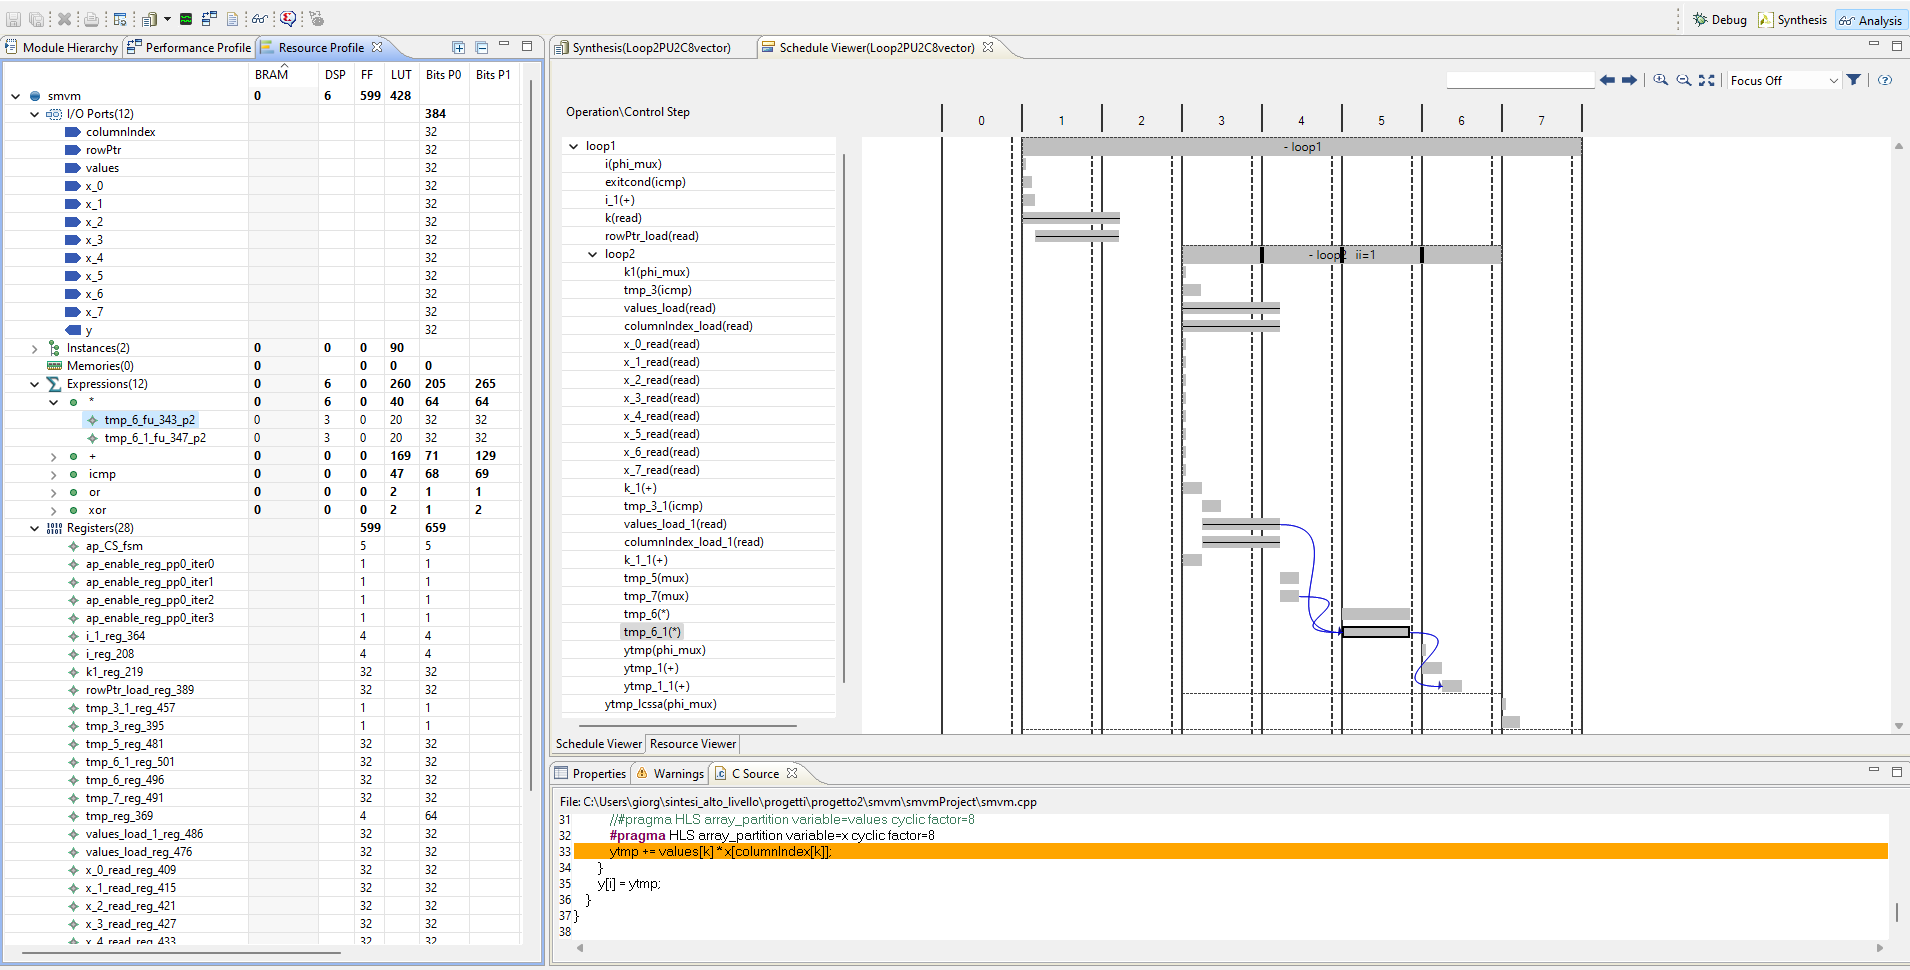
\includegraphics[width=1\textwidth]{solutions/s10/s10analysis.png}
	\caption{HLS Solution 10 Analysis}
\end{figure}

\begin{table}[H]
	\centering
	\begin{tabular}{|c|c|c|c|c|c|c|c|c|}
		\hline
		\multicolumn{1}{|c|}{\textbf{Solution}} & \multicolumn{1}{|c|}{RTL} & \multicolumn{1}{|c|}{Status} & \multicolumn{3}{c|}{\textbf{Latency}} & \multicolumn{3}{c|}{\textbf{Interval}} \\
		& &  & min & avg & max & min & avg & max \\
		\hline
		columnIndex, values, x & VHDL & Pass & 61 & 61 & 61 & NA & NA & NA \\
		\hline
		columnIndex & VHDL & Pass & 69 & 69 & 69 & NA & NA & NA \\
		\hline
		values & VHDL & Pass & 69 & 69 & 69 & NA & NA & NA \\
		\hline
		x & VHDL & Pass & 61 & 61 & 61 & NA & NA & NA \\
		\hline
	\end{tabular}
	\caption{HLS Solution 10 C/RTL Cosimulation Report }
	\label{tab:hls-solution-10-cosimulation-report}
\end{table}

Si può notare come l'utilizzazione delle risorse sia aumentata rispetto alle soluzioni 6 (loop2 Pipeline, Unroll=2, Cyclic=2) e 8 (loop2 Pipeline, Unroll=2, Cyclic=4). In particolare, considerando le soluzioni hardware corrispondenti al partizionamento di tutti e tre gli array, si evidenzia rispettivamente un aumento di circa l'$81\%$ e di circa il $66\%$ in corrispondenza delle slice rispetto alla soluzione 6 e 8, un aumento di circa il $77\%$ e di circa il $63\%$ in corrispondenza delle LUT, un aumento di circa il $127\%$ e di circa il $43\%$. 
\\
Per quanto riguarda le soluzioni hardware corrispondenti al partizionamento di columnIndex, rispetto alla soluzione 6 e 8, si registra rispettivamente un aumento di un'unità e una diminuzione di 2 slice, un aumento di nove unità e di 7 unità delle LUT, un aumento di 6 unità e di 4 unità dei FF. 
\\
Per quanto riguarda le solution corrispondenti al partitioning di values, rispetto alla soluzione 6 e 8, si registra rispettivamente un aumento di circa il $18\%$ e di circa il $27\%$ delle slice, un aumento di 15 unità e di circa il $25\%$ delle LUT, una diminuzione di 25 unità e un aumento di 3 unità dei FF. 
\\
Per quanto riguarda le soluzioni hardware corrispondenti al partizionamento di x, rispetto alla soluzione 6 e 8, si registra rispettivamente un aumento di circa il $44\%$ e di circa il $38\%$ delle slice, un aumento di circa il $24\%$ e di circa il $25\%$ delle LUT, un aumento di circa il $124\%$ e di circa il $42\%$ dei FF.

\begin{table}[H]
	\centering
	\begin{tabular}{|c|c|c|c|c|c|c|c|c|}
		\hline
		\textbf{Solution} & \textbf{SLICE} & \textbf{LUT} & \textbf{FF} & \textbf{DSP} & \textbf{BRAM} & \textbf{CP} & \textbf{CP} & \textbf{CP} \\
		& & & & & & \textbf{required} & \textbf{achieved} & \textbf{achieved}\\
		& & & & & & & \textbf{post-} & \textbf{post-}\\
		& & & & & & & \textbf{synthesis} & \textbf{implementation}\\
		\hline
		columnIndex, values, x  & 204 & 558 & 449 & 6 & 0 & 10 & 6.540 & 6.840 \\
		\hline
		columnIndex  & 83 & 268 & 230 & 6 & 0 & 10 & 7.496 & 8.115 \\
		\hline
		values  & 117 & 342 & 199 & 6 & 0 & 10 & 7.927 & 7.603 \\
		\hline
		x  & 143 & 311 & 444 & 6 & 0 & 10 & 6.540 & 6.790 \\
		\hline
	\end{tabular}
	\caption{HLS Solution 10 Export RTL Report}
	\label{tab:hls-solution-10-export-rtl-report}
\end{table}

Ovviamente questo aumento di utilizzazione delle risorse è dovuto all'incremento del fattore di partizionamento adottato nelle soluzioni hardware. Infatti, si evidenzia che il maggiore incremento delle risorse si ha rispetto alla soluzione 6 dove era previsto un fattore pari a 2 rispetto alla soluzione in questione dove il fattore di partitioning previsto è stato di 8.
\newpage

\subsection{Solution 11}
Considerando il codice utilizzato nella precedente solution, nella soluzione hardware in questione verrà utilizzata la direttiva di pipeline, di unrolling di fattore pari a 2 e la direttiva di partizionamento di tipologia block. Nello specifico, verranno analizzate le seguenti implementazioni relative al loop2:
\begin{itemize}
	\item Pipeline, Unroll=2, Block=8 (columnIndex, values, x)
	\item Pipeline, Unroll=2, Block=8 (columnIndex)
	\item Pipeline, Unroll=2, Block=8 (values)
	\item Pipeline, Unroll=2, Block=8 (x)
\end{itemize}

In particolare, è possibile evidenziare nel dettaglio le differenti soluzioni hardware nei seguenti allegati.
\lstinputlisting[language=C]{solutions/s11/definitions.h}
\lstinputlisting[language=C++]{solutions/s11/s11all3.cpp}
\lstinputlisting[language=C++]{solutions/s11/s11columnIndex.cpp}
\lstinputlisting[language=C++]{solutions/s11/s11values.cpp}
\lstinputlisting[language=C++]{solutions/s11/s11x.cpp}

Effettuando la sintesi si ottiene il seguente log.
\\
\textcolor{blue}{WARNING: [XFORM 203-105] Cannot partition array 'columnIndex' (smvmProject/smvm.cpp:11): indivisible factor 8 on dimension 1, which has 9 elements.}
\\
\textcolor{blue}{WARNING: [XFORM 203-105] Cannot partition array 'values' (smvmProject/smvm.cpp:11): indivisible factor 8 on dimension 1, which has 9 elements.}
\\
In particolare, la console sta segnalando che il tool non riesce a partizionare correttamente, tramite la tipologia block e il fattore 8 dichiarato, gli array columnIndex e values dal momento che presentano un numero di elementi che risulta essere non multiplo del fattore di array partitioning dichiarato. Pertanto, a tale proposito si modifica, di conseguenza, la variabile nnz, cioè il numero di elementi non nulli all'interno della matrice, nell'header. Nello specifico è stato scelto un valore pari a 16. Pertanto, ciò che ci si aspetta è che il tool divida tali array, columnIndex e values, in 8 sub-array aventi ognuno 2 elementi. Invece, per quanto riguarda l'array x, avente dimensione pari a 8, ci si aspetta che il tool lo divida in 8 sub-array da un elemento ognuno.

\lstinputlisting[language=C]{solutions/s11/headermodified.h}

Pertanto, effettuando la sintesi si ottiene il seguente report.

\begin{table}[H]
	\centering
	\begin{tabular}{|c|c|c|c|c|}
		\hline
		\textbf{Solution} & \textbf{Clock} & \textbf{Target} & \textbf{Estimated} & \textbf{Uncertainty} \\
		\hline
		columnIndex, values, x & ap\_clk & 10.00 & 8.510 & 1.25 \\
		\hline
		columnIndex & ap\_clk & 10.00 & 8.510 & 1.25 \\
		\hline
		values & ap\_clk & 10.00 & 8.510 & 1.25 \\
		\hline
		x & ap\_clk & 10.00 & 8.510 & 1.25 \\
		\hline
	\end{tabular}
	\caption{HLS Solution 11 Timing Summary (ns)}
	\label{tab:hls-solution-11-timing-summary}
\end{table}

\begin{table}[H]
	\centering
	\begin{tabular}{|c|c|c|c|c|}
		\hline
		\multicolumn{1}{|c|}{\textbf{Solution}} & \multicolumn{2}{|c|}{\textbf{Latency}} & \multicolumn{2}{|c|}{\textbf{Interval}} \\
		& min & max & min & max \\
		\hline
		columnIndex, values, x & 57 & 89 & 57 & 89 \\
		\hline
		columnIndex & 65 & 97 & 65 & 97 \\
		\hline
		values & 65 & 97 & 65 & 97 \\
		\hline
		x & 57 & 89 & 57 & 89 \\
		\hline
	\end{tabular}
	\caption{HLS Solution 11 Latency Summary (clock cycles)}
	\label{tab:hls-solution-11-latency-summary}
\end{table}

\begin{table}[H]
	\centering
	\begin{tabular}{|c|c|c|c|c|c|c|c|c|c|}
		\hline
		\multicolumn{1}{|c|}{\textbf{Solution}} & \multicolumn{1}{|c|}{Loop Name} & \multicolumn{2}{|c|}{\textbf{Latency}} & \multicolumn{1}{c|}{\textbf{Iteration Latency}} & \multicolumn{2}{c|}{\textbf{Initiation Interval}} & \multicolumn{1}{c|}{\textbf{Trip}}  \\
		&  & min & max & & achieved & target & \textbf{Count} \\
		\hline
		columnIndex, values, x & - loop1 & 56 & 88 & 7$\sim$11 & - & - & 8 \\
		& + loop2 & 3 & 7 & 4 & 1 & 1 & 0$\sim$4 \\
		\hline
		columnIndex & - loop1 & 64 & 96 & 8$\sim$12 & - & - & 8 \\
		& + loop2 & 4 & 8 & 5 & 1 & 1 & 0$\sim$4 \\
		\hline
		values & - loop1 & 64 & 96 & 8$\sim$12 & - & - & 8 \\
		& + loop2 & 4 & 8 & 5 & 1 & 1 & 0$\sim$4 \\
		\hline
		x & - loop1 & 56 & 88 & 7$\sim$11 & - & - & 8 \\
		& + loop2 & 3 & 7 & 4 & 1 & 1 & 0$\sim$4 \\
		\hline
	\end{tabular}
	\caption{HLS Solution 11 Latency Loops Summary }
	\label{tab:hls-solution-11-loop-summary}
\end{table}

\begin{table}[H]
	\centering
	\begin{tabular}{|c|c|c|c|c|}
		\hline
		\textbf{Solution} & \textbf{BRAM\_18K} & \textbf{DSP48E} & \textbf{FF} & \textbf{LUT} \\
		\hline
		columnIndex, values, x & 0 & 6 & 789 & 674 \\
		\hline
		columnIndex & 0 & 6 & 536 & 503 \\
		\hline
		values & 0 & 6 & 597 & 503 \\
		\hline
		x & 0 & 6 & 727 & 492 \\
		\hline
	\end{tabular}
	\caption{HLS Solution 11 Utilization Estimates [\#]}
	\label{tab:hls-solution-11-utilization-report}
\end{table}

\begin{table}[H]
	\centering
	\begin{tabular}{|c|c|c|c|c|c|c|c|c|}
		\hline
		\multicolumn{1}{|c|}{\textbf{Solution}} & \multicolumn{1}{|c|}{RTL} & \multicolumn{1}{|c|}{Status} & \multicolumn{3}{c|}{\textbf{Latency}} & \multicolumn{3}{c|}{\textbf{Interval}} \\
		& &  & min & avg & max & min & avg & max \\
		\hline
		columnIndex, values, x & VHDL & Pass & 64 & 64 & 64 & NA & NA & NA \\
		\hline
		columnIndex & VHDL & Pass & 72 & 72 & 72 & NA & NA & NA \\
		\hline
		values & VHDL & Pass & 72 & 72 & 72 & NA & NA & NA \\
		\hline
		x & VHDL & Pass & 64 & 64 & 64 & NA & NA & NA \\
		\hline
	\end{tabular}
	\caption{HLS Solution 11 C/RTL Cosimulation Report }
	\label{tab:hls-solution-11-cosimulation-report}
\end{table}

Si può notare come, rispetto alla solution 10 dove era stato applicato un partitioning dello stesso fattore ma di tipologia cyclic, l'utilizzazione delle risorse in corrispondenza del solo partizionamento dell'array x non cambia dal momento che è stata solo modificata il valore della variabile nnz, cioè la dimensione degli array columnIndex e values.

\begin{table}[H]
	\centering
	\begin{tabular}{|c|c|c|c|c|c|c|c|c|}
		\hline
		\textbf{Solution} & \textbf{SLICE} & \textbf{LUT} & \textbf{FF} & \textbf{DSP} & \textbf{BRAM} & \textbf{CP} & \textbf{CP} & \textbf{CP} \\
		& & & & & & \textbf{required} & \textbf{achieved} & \textbf{achieved}\\
		& & & & & & & \textbf{post-} & \textbf{post-}\\
		& & & & & & & \textbf{synthesis} & \textbf{implementation}\\
		\hline
		columnIndex, values, x  & 179 & 454 & 450 & 6 & 0 & 10 & 6.541 & 6.677 \\
		\hline
		columnIndex  & 90 & 267 & 227 & 6 & 0 & 10 & 7.489 & 7.664 \\
		\hline
		values  & 122 & 391 & 232 & 6 & 0 & 10 & 7.506 & 7.768 \\
		\hline
		x  & 143 & 311 & 444 & 6 & 0 & 10 & 6.540 & 6.790 \\
		\hline
	\end{tabular}
	\caption{HLS Solution 11 Export RTL Report}
	\label{tab:hls-solution-11-export-rtl-report}
\end{table}
\newpage
	\newpage
	
	\section{Conclusions}
	

\begin{table}[H]
	\centering
	\begin{tabular}{|l|c|c|c|c|c|c|c|c|}
		\hline
		\multicolumn{1}{|c|}{\textbf{Solution}} & \multicolumn{1}{|c|}{RTL} & \multicolumn{1}{|c|}{Status} & \multicolumn{3}{c|}{\textbf{Latency}} & \multicolumn{3}{c|}{\textbf{Interval}} \\
		& &  & min & avg & max & min & avg & max \\
		\hline
		1 & VHDL & Pass & 58 & 58 & 58 & NA & NA & NA \\
		\hline
		2 & VHDL & Pass & 38 & 38 & 38 & NA & NA & NA \\
		\hline
		3 & VHDL & Pass & 58 & 58 & 58 & NA & NA & NA \\
		\hline
		4 & VHDL & Pass & 56 & 56 & 56 & NA & NA & NA \\
		\hline
		5 & VHDL & Pass & 37 & 37 & 37 & NA & NA & NA \\
		\hline
		6 &  &  &  &  &  &  &  &  \\
		\tabitem columnIndex, values, x & VHDL & Pass & 37 & 37 & 37 & NA & NA & NA \\
		\tabitem columnIndex & VHDL & Pass & 37 & 37 & 37 & NA & NA & NA \\
		\tabitem values & VHDL & Pass & 37 & 37 & 37 & NA & NA & NA \\
		\tabitem x & VHDL & Pass & 37 & 37 & 37 & NA & NA & NA \\
		\hline
		7 & VHDL & Pass & 29 & 29 & 29 & NA & NA & NA \\
		\hline
		8 &  &  &  &  &  &  &  &  \\
		\tabitem columnIndex, values, x & VHDL & Pass & 33 & 33 & 33 & NA & NA & NA \\
		\tabitem columnIndex & VHDL & Pass & 37 & 37 & 37 & NA & NA & NA \\
		\tabitem values & VHDL & Pass & 37 & 37 & 37 & NA & NA & NA \\
		\tabitem x & VHDL & Pass & 33 & 33 & 33 & NA & NA & NA \\
		\hline
		9 & VHDL & Pass & 30 & 30 & 30 & NA & NA & NA \\
		\hline
		10 &  &  &  &  &  &  &  &  \\
		\tabitem columnIndex, values, x & VHDL & Pass & 61 & 61 & 61 & NA & NA & NA \\
		\tabitem columnIndex & VHDL & Pass & 69 & 69 & 69 & NA & NA & NA \\
		\tabitem values & VHDL & Pass & 69 & 69 & 69 & NA & NA & NA \\
		\tabitem x & VHDL & Pass & 61 & 61 & 61 & NA & NA & NA \\
		\hline
		11 &  &  &  &  &  &  &  &  \\
		\tabitem columnIndex, values, x & VHDL & Pass & 64 & 64 & 64 & NA & NA & NA \\
		\tabitem columnIndex & VHDL & Pass & 72 & 72 & 72 & NA & NA & NA \\
		\tabitem values & VHDL & Pass & 72 & 72 & 72 & NA & NA & NA \\
		\tabitem x & VHDL & Pass & 64 & 64 & 64 & NA & NA & NA \\
		\hline
	\end{tabular}
	\caption{HLS Conclusions C/RTL Cosimulation Report }
	\label{tab:hls-conclusions-cosimulation-report}
\end{table}

\begin{filecontents*}{latency.csv}
	Solution,Min,Avg,Max
	1,58,58,58
	2,38,38,38
	3,58,58,58
	4,56,56,56
	5,37,37,37
	6a,37,37,37
	6b,37,37,37
	6c,37,37,37
	6d,37,37,37
	7,29,29,29
	8a,33,33,33
	8b,37,37,37
	8c,37,37,37
	8d,33,33,33
	9,30,30,30
	10a,61,61,61
	10b,69,69,69
	10c,69,69,69
	10d,61,61,61
	11a,64,64,64
	11b,72,72,72
	11c,72,72,72
	11d,64,64,64
\end{filecontents*}

\begin{figure}
	\begin{tikzpicture}
		\begin{axis}[
			symbolic x coords={1, 2, 3, 4, 5, 6a, 6b, 6c, 6d, 7, 8a, 8b, 8c, 8d, 9, 10a, 10b, 10c, 10d, 11a, 11b, 11c, 11d},
			xtick=data,
			ymin=0,
			ymax=80,
			ylabel={Latency},
			xlabel={Solution},
			legend style={at={(0.5,-0.20)}, anchor=north, legend columns=-1},
			width=1\textwidth,
			height=0.7\textwidth,
			xticklabel style={rotate=90, anchor=east},
			]
			\addplot table [x=Solution, y=Min, col sep=comma] {latency.csv};
			\addplot table [x=Solution, y=Avg, col sep=comma] {latency.csv};
			\addplot table [x=Solution, y=Max, col sep=comma] {latency.csv};
			\legend{Min,Avg,Max}
		\end{axis}
	\end{tikzpicture}
	\caption{Latency measurements for different solutions}
	\label{fig:latency-measurements}
\end{figure}





\begin{table}[H]
	\centering
	\begin{tabular}{|l|c|c|c|c|c|}
		\hline
		\textbf{Solution} & \textbf{SLICE} & \textbf{LUT} & \textbf{FF} & \textbf{DSP} & \textbf{BRAM} \\
		\hline
		1 & 48 & 93 & 161 & 3 & 0 \\
		\hline
		2 & 38 & 115 & 139 & 3 & 0 \\
		\hline
		3 & 48 & 94 & 161 & 3 & 0 \\
		\hline
		4 & 83 & 186 & 292 & 3 & 0 \\
		\hline
		5 & 69 & 184 & 196 & 6 & 0 \\
		\hline
		6 &  &  &  &  & \\
		\tabitem columnIndex, values, x & 113 & 316 & 198 & 6 & 0 \\
		\tabitem columnIndex & 84 & 259 & 224 & 6 & 0 \\
		\tabitem values & 99 & 327 & 224 & 6 & 0 \\
		\tabitem x & 99 & 250 & 198 & 6 & 0 \\
		\hline
		7 & 314 & 915 & 297 & 12 & 0 \\
		\hline
		8 &  &  &  &  &  \\
		\tabitem columnIndex, values, x & 123 & 343 & 315 & 6 & 0 \\
		\tabitem columnIndex & 85 & 261 & 226 & 6 & 0 \\
		\tabitem values & 92 & 274 & 196 & 6 & 0 \\
		\tabitem x & 104 & 248 & 313 & 6 & 0 \\
		\hline
		9 & 75 & 248 & 131 & 3 & 0 \\
		\hline
		10 &  &  &  &  &  \\
		\tabitem columnIndex, values, x & 204 & 558 & 449 & 6 & 0 \\
		\tabitem columnIndex & 83 & 268 & 230 & 6 & 0 \\
		\tabitem values & 117 & 342 & 199 & 6 & 0 \\
		\tabitem x & 143 & 311 & 444 & 6 & 0 \\
		\hline
		11 &  &  &  &  &  \\
		\tabitem columnIndex, values, x & 179 & 454 & 450 & 6 & 0 \\
		\tabitem columnIndex & 90 & 267 & 227 & 6 & 0 \\
		\tabitem values & 122 & 391 & 232 & 6 & 0 \\
		\tabitem x & 143 & 311 & 444 & 6 & 0 \\
		\hline
	\end{tabular}
	\caption{HLS Conclusions Export RTL Report}
	\label{tab:hls-conclusions-export-rtl-report}
\end{table}

\begin{filecontents}{utilization.csv}
	Solution,SLICE,LUT,FF,DSP,BRAM
	1,48,93,161,3,0
	2,38,115,139,3,0
	3,48,94,161,3,0
	4,83,186,292,3,0
	5,69,184,196,6,0
	6a,113,316,198,6,0
	6b,84,259,224,6,0
	6c,99,327,224,6,0
	6d,99,250,198,6,0
	7,314,915,297,12,0
	8a,123,343,315,6,0
	8b,85,261,226,6,0
	8c,92,274,196,6,0
	8d,104,248,313,6,0
	9,75,248,131,3,0
	10a,204,558,449,6,0
	10b,83,268,230,6,0
	10c,117,342,199,6,0
	10d,143,311,444,6,0
	11a,179,454,450,6,0
	11b,90,267,227,6,0
	11c,122,391,232,6,0
	11d,143,311,444,6,0
\end{filecontents}

\begin{figure}
	\centering
	\begin{tikzpicture}
		\begin{axis}[
			symbolic x coords={1, 2, 3, 4, 5, 6a, 6b, 6c, 6d, 7, 8a, 8b, 8c, 8d, 9, 10a, 10b, 10c, 10d, 11a, 11b, 11c, 11d},
			xtick=data,
			xlabel={Solution},
			ylabel={\#},
			xticklabel style={rotate=90, anchor=east},
			width=1\textwidth,
			height=0.7\textwidth,
			enlarge x limits=0.05,
			legend style={at={(0.5,-0.15)}, anchor=north,legend columns=-1}
			]
			\addplot table [x=Solution, y=SLICE, col sep=comma] {utilization.csv};
			\addplot table [x=Solution, y=LUT, col sep=comma] {utilization.csv};
			\addplot table [x=Solution, y=FF, col sep=comma] {utilization.csv};
			\addplot table [x=Solution, y=DSP, col sep=comma] {utilization.csv};
			\addplot table [x=Solution, y=BRAM, col sep=comma] {utilization.csv};
			\legend{SLICE, LUT, FF, DSP, BRAM}
		\end{axis}
	\end{tikzpicture}
	\caption{Utilization Export RTL Plot}
	\label{fig:utilization-export-rtl-plot}
\end{figure}
	
	\newpage
	
\end{document}